% Options for packages loaded elsewhere
\PassOptionsToPackage{unicode}{hyperref}
\PassOptionsToPackage{hyphens}{url}
\PassOptionsToPackage{dvipsnames,svgnames,x11names}{xcolor}
%
\documentclass[
  11pt,
  article]{jss}

\usepackage{amsmath,amssymb}
\usepackage{iftex}
\ifPDFTeX
  \usepackage[T1]{fontenc}
  \usepackage[utf8]{inputenc}
  \usepackage{textcomp} % provide euro and other symbols
\else % if luatex or xetex
  \usepackage{unicode-math}
  \defaultfontfeatures{Scale=MatchLowercase}
  \defaultfontfeatures[\rmfamily]{Ligatures=TeX,Scale=1}
\fi
\usepackage{lmodern}
\ifPDFTeX\else  
    % xetex/luatex font selection
\fi
% Use upquote if available, for straight quotes in verbatim environments
\IfFileExists{upquote.sty}{\usepackage{upquote}}{}
\IfFileExists{microtype.sty}{% use microtype if available
  \usepackage[]{microtype}
  \UseMicrotypeSet[protrusion]{basicmath} % disable protrusion for tt fonts
}{}
\makeatletter
\@ifundefined{KOMAClassName}{% if non-KOMA class
  \IfFileExists{parskip.sty}{%
    \usepackage{parskip}
  }{% else
    \setlength{\parindent}{0pt}
    \setlength{\parskip}{6pt plus 2pt minus 1pt}}
}{% if KOMA class
  \KOMAoptions{parskip=half}}
\makeatother
\usepackage{xcolor}
\setlength{\emergencystretch}{3em} % prevent overfull lines
\setcounter{secnumdepth}{-\maxdimen} % remove section numbering
% Make \paragraph and \subparagraph free-standing
\makeatletter
\ifx\paragraph\undefined\else
  \let\oldparagraph\paragraph
  \renewcommand{\paragraph}{
    \@ifstar
      \xxxParagraphStar
      \xxxParagraphNoStar
  }
  \newcommand{\xxxParagraphStar}[1]{\oldparagraph*{#1}\mbox{}}
  \newcommand{\xxxParagraphNoStar}[1]{\oldparagraph{#1}\mbox{}}
\fi
\ifx\subparagraph\undefined\else
  \let\oldsubparagraph\subparagraph
  \renewcommand{\subparagraph}{
    \@ifstar
      \xxxSubParagraphStar
      \xxxSubParagraphNoStar
  }
  \newcommand{\xxxSubParagraphStar}[1]{\oldsubparagraph*{#1}\mbox{}}
  \newcommand{\xxxSubParagraphNoStar}[1]{\oldsubparagraph{#1}\mbox{}}
\fi
\makeatother


\providecommand{\tightlist}{%
  \setlength{\itemsep}{0pt}\setlength{\parskip}{0pt}}\usepackage{longtable,booktabs,array}
\usepackage{calc} % for calculating minipage widths
% Correct order of tables after \paragraph or \subparagraph
\usepackage{etoolbox}
\makeatletter
\patchcmd\longtable{\par}{\if@noskipsec\mbox{}\fi\par}{}{}
\makeatother
% Allow footnotes in longtable head/foot
\IfFileExists{footnotehyper.sty}{\usepackage{footnotehyper}}{\usepackage{footnote}}
\makesavenoteenv{longtable}
\usepackage{graphicx}
\makeatletter
\def\maxwidth{\ifdim\Gin@nat@width>\linewidth\linewidth\else\Gin@nat@width\fi}
\def\maxheight{\ifdim\Gin@nat@height>\textheight\textheight\else\Gin@nat@height\fi}
\makeatother
% Scale images if necessary, so that they will not overflow the page
% margins by default, and it is still possible to overwrite the defaults
% using explicit options in \includegraphics[width, height, ...]{}
\setkeys{Gin}{width=\maxwidth,height=\maxheight,keepaspectratio}
% Set default figure placement to htbp
\makeatletter
\def\fps@figure{htbp}
\makeatother

\usepackage{booktabs}
\usepackage{longtable}
\usepackage{array}
\usepackage{multirow}
\usepackage{wrapfig}
\usepackage{float}
\usepackage{pdflscape}
\usepackage{tabu}
\usepackage{threeparttable}
\usepackage{threeparttablex}
\usepackage[normalem]{ulem}
\usepackage[utf8]{inputenc}
\usepackage{makecell}
\usepackage{xcolor}
\usepackage{placeins}


\newtheorem{definition}{Definition}
\usepackage{orcidlink,thumbpdf,lmodern}

\newcommand{\class}[1]{`\code{#1}'}
\newcommand{\fct}[1]{\code{#1()}}
\makeatletter
\@ifpackageloaded{tcolorbox}{}{\usepackage[skins,breakable]{tcolorbox}}
\@ifpackageloaded{fontawesome5}{}{\usepackage{fontawesome5}}
\definecolor{quarto-callout-color}{HTML}{909090}
\definecolor{quarto-callout-note-color}{HTML}{0758E5}
\definecolor{quarto-callout-important-color}{HTML}{CC1914}
\definecolor{quarto-callout-warning-color}{HTML}{EB9113}
\definecolor{quarto-callout-tip-color}{HTML}{00A047}
\definecolor{quarto-callout-caution-color}{HTML}{FC5300}
\definecolor{quarto-callout-color-frame}{HTML}{acacac}
\definecolor{quarto-callout-note-color-frame}{HTML}{4582ec}
\definecolor{quarto-callout-important-color-frame}{HTML}{d9534f}
\definecolor{quarto-callout-warning-color-frame}{HTML}{f0ad4e}
\definecolor{quarto-callout-tip-color-frame}{HTML}{02b875}
\definecolor{quarto-callout-caution-color-frame}{HTML}{fd7e14}
\makeatother
\makeatletter
\@ifpackageloaded{caption}{}{\usepackage{caption}}
\AtBeginDocument{%
\ifdefined\contentsname
  \renewcommand*\contentsname{Table of contents}
\else
  \newcommand\contentsname{Table of contents}
\fi
\ifdefined\listfigurename
  \renewcommand*\listfigurename{List of Figures}
\else
  \newcommand\listfigurename{List of Figures}
\fi
\ifdefined\listtablename
  \renewcommand*\listtablename{List of Tables}
\else
  \newcommand\listtablename{List of Tables}
\fi
\ifdefined\figurename
  \renewcommand*\figurename{Figure}
\else
  \newcommand\figurename{Figure}
\fi
\ifdefined\tablename
  \renewcommand*\tablename{Table}
\else
  \newcommand\tablename{Table}
\fi
}
\@ifpackageloaded{float}{}{\usepackage{float}}
\floatstyle{ruled}
\@ifundefined{c@chapter}{\newfloat{codelisting}{h}{lop}}{\newfloat{codelisting}{h}{lop}[chapter]}
\floatname{codelisting}{Listing}
\newcommand*\listoflistings{\listof{codelisting}{List of Listings}}
\makeatother
\makeatletter
\makeatother
\makeatletter
\@ifpackageloaded{caption}{}{\usepackage{caption}}
\@ifpackageloaded{subcaption}{}{\usepackage{subcaption}}
\makeatother
\makeatletter
\@ifpackageloaded{tcolorbox}{}{\usepackage[skins,breakable]{tcolorbox}}
\makeatother
\makeatletter
\@ifundefined{shadecolor}{\definecolor{shadecolor}{rgb}{.97, .97, .97}}{}
\makeatother
\makeatletter
\makeatother
\makeatletter
\ifdefined\Shaded\renewenvironment{Shaded}{\begin{tcolorbox}[frame hidden, enhanced, boxrule=0pt, borderline west={3pt}{0pt}{shadecolor}, interior hidden, breakable, sharp corners]}{\end{tcolorbox}}\fi
\makeatother
\ifLuaTeX
  \usepackage{selnolig}  % disable illegal ligatures
\fi
\usepackage{bookmark}

\IfFileExists{xurl.sty}{\usepackage{xurl}}{} % add URL line breaks if available
\urlstyle{same} % disable monospaced font for URLs
\hypersetup{
  pdftitle={Making, Updating, and Querying Causal Models using CausalQueries},
  pdfauthor={Till Tietz; Lily Medina; Georgiy Syunyaev; Macartan Humphreys},
  colorlinks=true,
  linkcolor={blue},
  filecolor={Maroon},
  citecolor={Blue},
  urlcolor={Blue},
  pdfcreator={LaTeX via pandoc}}

%% -- Article metainformation (author, title, ...) -----------------------------

%% Author information
\author{Till Tietz~\orcidlink{0000-0002-2916-9059}\\Humboldt
University \And Lily Medina~\orcidlink{0009-0004-2423-524X}\\University
of California, Berkeley \AND Georgiy
Syunyaev~\orcidlink{0000-0002-4391-6313}\\Vanderbilt
University \And Macartan Humphreys~\orcidlink{0000-0001-7029-2326}\\WZB}
\Plainauthor{Till Tietz, Lily Medina, Georgiy Syunyaev, Macartan
Humphreys} %% comma-separated

\title{Making, Updating, and Querying Causal Models using
\texttt{CausalQueries}}
\Plaintitle{Making, Updating, and Querying Causal Models using
CausalQueries} %% without formatting

%% an abstract and keywords
\Abstract{The \proglang{R} package \texttt{CausalQueries} can be used to
make, update, and query causal models defined on binary nodes. Users
provide a causal statement of the form
\texttt{X\ -\textgreater{}\ M\ \textless{}-\ Y;\ M\ \textless{}-\textgreater{}\ Y}
which is interpreted as a structural causal model over a collection of
binary nodes. Then \texttt{CausalQueries} allows users to (1) identify
the set of principal strata---causal types---required to characterize
all possible causal relations between nodes that are consistent with the
causal statement (2) determine a set of parameters needed to
characterize distributions over these causal types (3) update beliefs
over distributions of causal types, using a \texttt{stan} model plus
data, and (4) pose a wide range of causal queries of the model, using
either the prior distribution, the posterior distribution, or a
user-specified candidate vector of parameters.}

%% at least one keyword must be supplied
\Keywords{causal model, Bayesian updating, DAG, Stan}

%% publication information
%% NOTE: Typically, this can be left commented and will be filled out by the technical editor
%% \Volume{50}
%% \Issue{9}
%% \Month{June}
%% \Year{2012}
%% \Submitdate{2012-06-04}
%% \Acceptdate{2012-06-04}
%% \setcounter{page}{1}
%% \Pages{1--xx}

%% The address of (at least) one author should be given
%% in the following format:
\Address{
Till Tietz\\
Humboldt University\\
Berlin Germany\\
E-mail: \email{ttietz2014@gmail.com}\\
URL: \url{https://github.com/till-tietz}\\
\\~
Lily Medina\\
University of California, Berkeley\\
E-mail: \email{lily.medina@berkeley.edu}\\
URL: \url{https:/lilymedina.github.io/}\\
\\~
Georgiy Syunyaev\\
Vanderbilt University\\
E-mail: \email{g.syunyaev@vanderbilt.edu}\\
URL: \url{https://gsyunyaev.com/}\\
\\~
Macartan Humphreys\\
WZB, IPI\\
Reichpietschufer 50\\
Berlin Germany\\
E-mail: \email{macartan.humphreys@wzb.eu}\\
URL: \url{https://macartan.github.io/}\\
\\~

}

\begin{document}
\maketitle

\section{Introduction: Causal models}\label{sec-intro}

\texttt{CausalQueries} is an \proglang{R} package that lets users make,
update, and query causal models. Users provide a structural causal model
in the form of a statement that reports a set of binary variables and
the relations of causal ancestry between them. Once such a statement is
provided to \texttt{make\_model()}, \texttt{CausalQueries} generates a
parameter vector that fully describes a probability distribution over
all possible types of causal relations between variables (``causal
types''). Given a prior distribution over parameters---equivalently,
over causal models consistent with the structural model--- and data on
some or all nodes, \texttt{update\_model()} deploys a Stan
\citep{carpenter_stan_2017} model to generate a posterior distribution
over causal models. The function \texttt{query\_model()} can then be
used to ask a wide range of causal queries, using either the prior
distribution, the posterior distribution, or a user-specified candidate
vector of parameters.

In the next section we provide a motivating example. We then describe
how the package relates to existing available software.
Section~\ref{sec-theory} gives an overview of the statistical model
behind the package. Section~\ref{sec-make}, Section~\ref{sec-update},
and Section~\ref{sec-query} then describe, in turn, the functionality
for making, updating, and querying causal models. We provide further
computation details in the final section.

\section{Motivating example}\label{motivating-example}

Before providing details on package functionality, we illustrate the
three core functions of the package by showing how to use
\texttt{CausalQueries} to replicate the analysis in
\citetext{\citealp{chickering_clinicians_1996}; \citealp[see
also][]{humphreys_integrated_2023}}. \citet{chickering_clinicians_1996}
seek to draw inferences on causal effects in the presence of imperfect
compliance. We have access to an instrument \(Z\) (a randomly assigned
prescription for cholesterol medication), which is a cause of \(X\)
(treatment uptake) but otherwise unrelated to \(Y\) (cholesterol). We
imagine we are interested in three specific queries. The first is the
average causal effect of \(X\) on \(Y\). The second is the average
effect for units for which \(X=0\) and \(Y=0\). The last is the average
effect for ``compliers'': units for which \(X\) responds positively to
\(Z\). Thus two of these queries are conditional queries, with one
conditional on a counterfactual quantity.

The data on \(Z\), \(X\), and \(Y\) is given in
\citet{chickering_clinicians_1996} and is also included in the
\texttt{CausalQueries} package. The data is complete for all units and
looks as follows:

\begin{verbatim}
R> data("lipids_data")
R> 
R> lipids_data
\end{verbatim}

\begin{verbatim}
#>    event strategy count
#> 1 Z0X0Y0      ZXY   158
#> 2 Z1X0Y0      ZXY    52
#> 3 Z0X1Y0      ZXY     0
#> 4 Z1X1Y0      ZXY    23
#> 5 Z0X0Y1      ZXY    14
#> 6 Z1X0Y1      ZXY    12
#> 7 Z0X1Y1      ZXY     0
#> 8 Z1X1Y1      ZXY    78
\end{verbatim}

This data is reported in ``compact form,'' meaning it records the number
of units (``count'') that display each possible pattern of outcomes on
the three variables (``event''). The ``strategy'' column records the set
of variables for which data has been recorded. In this illustration the
data is complete and so the implied strategy is \texttt{ZXY} for all
units.

\texttt{CausalQueries} then allows users to create the model, input
data, and update the model as follows:

\begin{verbatim}
R> lipids_model <-  
+  make_model("Z -> X -> Y; X <-> Y") |>
+  update_model(lipids_data)
\end{verbatim}

Finally, the model can then be queried:

\begin{verbatim}
R> lipids_queries <- 
+  lipids_model  |>
+  query_model(query = "Y[X=1] - Y[X=0]",
+              given = c("All",  "X==0 & Y==0", "X[Z=1] > X[Z=0]"),
+              using = "posteriors") 
\end{verbatim}

Here three distinct queries are posed, with the queries differing in the
type of conditioning imposed.

The output is a data frame with estimates, posterior standard
deviations, and credibility intervals. Table~\ref{tbl-lipids} shows the
output from the analysis of the lipids data. Rows 1 and 2 in the table
replicate results in \citet{chickering_clinicians_1996}; row 3 returns
inferences for complier average effects.

\begin{longtable}[t]{cccccc}

\caption{\label{tbl-lipids}Replication of
\citet{chickering_clinicians_1996}.}

\tabularnewline

\toprule
query & given & mean & sd & cred.low & cred.high\\
\midrule
Y[X=1] - Y[X=0] & - & 0.55 & 0.10 & 0.37 & 0.73\\
Y[X=1] - Y[X=0] & X==0 \& Y==0 & 0.64 & 0.15 & 0.37 & 0.89\\
Y[X=1] - Y[X=0] & X[Z=1] > X[Z=0] & 0.70 & 0.05 & 0.59 & 0.80\\
\bottomrule

\end{longtable}

As we describe below, the same basic procedure of making, updating, and
querying models, can be used (up to computational constraints) for
arbitrary causal models, for different types of data structures, and for
all causal queries that can be posed of the causal model.

\section{Connections to existing
packages}\label{connections-to-existing-packages}

The literature on causal inference and its software ecosystem is large,
spanning the social and natural sciences as well as computer science and
applied mathematics. Here we contextualize the scope and functionality
of \texttt{CausalQueries} within the subset of the causal inference
domain addressing the evaluation of causal queries on causal models
encoded as directed acyclic graphs (DAGs) or structural equation models
(SEMs). Table~\ref{tbl-software} provides an overview of relevant
software and discusses key connections, advantages and disadvantages
with respect to \texttt{CausalQueries}.

\begin{longtable}[]{@{}
  >{\raggedright\arraybackslash}p{(\columnwidth - 8\tabcolsep) * \real{0.1800}}
  >{\raggedright\arraybackslash}p{(\columnwidth - 8\tabcolsep) * \real{0.1900}}
  >{\raggedright\arraybackslash}p{(\columnwidth - 8\tabcolsep) * \real{0.1000}}
  >{\raggedright\arraybackslash}p{(\columnwidth - 8\tabcolsep) * \real{0.1700}}
  >{\raggedright\arraybackslash}p{(\columnwidth - 8\tabcolsep) * \real{0.3600}}@{}}
\caption{Related software.}\label{tbl-software}\tabularnewline
\toprule\noalign{}
\begin{minipage}[b]{\linewidth}\raggedright
Software
\end{minipage} & \begin{minipage}[b]{\linewidth}\raggedright
Source
\end{minipage} & \begin{minipage}[b]{\linewidth}\raggedright
Language
\end{minipage} & \begin{minipage}[b]{\linewidth}\raggedright
Availability
\end{minipage} & \begin{minipage}[b]{\linewidth}\raggedright
Scope
\end{minipage} \\
\midrule\noalign{}
\endfirsthead
\toprule\noalign{}
\begin{minipage}[b]{\linewidth}\raggedright
Software
\end{minipage} & \begin{minipage}[b]{\linewidth}\raggedright
Source
\end{minipage} & \begin{minipage}[b]{\linewidth}\raggedright
Language
\end{minipage} & \begin{minipage}[b]{\linewidth}\raggedright
Availability
\end{minipage} & \begin{minipage}[b]{\linewidth}\raggedright
Scope
\end{minipage} \\
\midrule\noalign{}
\endhead
\bottomrule\noalign{}
\endlastfoot
\texttt{causalnex} & \citet{beaumont_causalnex_2021} & \proglang{Python}
& \begin{minipage}[t]{\linewidth}\raggedright
\begin{itemize}
\tightlist
\item
  pip
\end{itemize}
\end{minipage} & \begin{minipage}[t]{\linewidth}\raggedright
\begin{itemize}
\tightlist
\item
  causal structure learning
\item
  querying marginal distributions
\item
  discrete data
\end{itemize}
\end{minipage} \\
\texttt{pclag} & \citet{kalisch_causal_2012} & \proglang{R} &
\begin{minipage}[t]{\linewidth}\raggedright
\begin{itemize}
\tightlist
\item
  CRAN
\item
  GitHub
\end{itemize}
\end{minipage} & \begin{minipage}[t]{\linewidth}\raggedright
\begin{itemize}
\tightlist
\item
  causal structure learning
\item
  ATEs under linear conditional expectations, no hidden selection
\end{itemize}
\end{minipage} \\
\texttt{DoWhy} & \citet{dowhy} & \proglang{Python} &
\begin{minipage}[t]{\linewidth}\raggedright
\begin{itemize}
\tightlist
\item
  pip
\end{itemize}
\end{minipage} & \begin{minipage}[t]{\linewidth}\raggedright
\begin{itemize}
\tightlist
\item
  identification
\item
  average and conditional causal effects
\item
  robustness checks
\end{itemize}
\end{minipage} \\
\texttt{autobounds} & \citet{duarte_automated_2023} & \proglang{Python}
& \begin{minipage}[t]{\linewidth}\raggedright
\begin{itemize}
\tightlist
\item
  Docker
\item
  GitHub
\end{itemize}
\end{minipage} & \begin{minipage}[t]{\linewidth}\raggedright
\begin{itemize}
\tightlist
\item
  bounding causal effects
\item
  partial identification
\item
  DAG canonicalization
\item
  binary data
\end{itemize}
\end{minipage} \\
\texttt{causaloptim} & \citet{sachs_general_2023} & \proglang{R} &
\begin{minipage}[t]{\linewidth}\raggedright
\begin{itemize}
\tightlist
\item
  CRAN
\item
  GitHub
\end{itemize}
\end{minipage} & \begin{minipage}[t]{\linewidth}\raggedright
\begin{itemize}
\tightlist
\item
  bounding causal effects
\item
  non-identified queries
\item
  binary data
\end{itemize}
\end{minipage} \\
\end{longtable}

\texttt{causalnex} is a comprehensive software that offers a suite of
functions for the discovery and querying of causal models. Like
\texttt{CausalQueries}, it uses Bayesian methods and allows users to use
``\texttt{do} calculus'' \citep{pearl_causality_2009}. The parameters of
focus are conditional probability distribution tables rather than
principal strata (causal types). This approach limits the types of
queries that can be posed and the kinds of expert information that can
be incorporated. For instance, knowledge of conditional probability
distributions are not sufficient to make claims about (or provide priors
with respect to) effect monotonicity, complier effects, or the
``probability of causation'' \citep{dawid2017probability}. However it
makes it possible to address simple queries efficiently with much larger
models.

Like \texttt{causalnex}, \texttt{pclag} places particular emphasis on
learning about causal structures, utilizing the resultant DAGs to
recover average treatment effects (ATEs) across all learned
Markov-equivalent classes implied by observed data that satisfy
linearity of conditional expectations. This approach again is more
restrictive than \texttt{CausalQueries} in the queries it allows.

\texttt{DoWhy} is a feature-rich framework that emphasizes causal
identification, causal effect estimation, and assumption validation.
Given a user-specified DAG, it deploys do-calculus to find expressions
that identify desired causal-effects via Back-door, Front-door, IV and
mediation identification criteria and leverages the identified
expression and standard estimators to estimate the desired estimand.
Following estimation, \texttt{DoWhy} deploys a comprehensive refutation
engine implementing a large set of robustness tests. While this approach
allows it to efficiently handle varied data types on large causal
models, the decision to not parameterize the DAG itself places
substantial limitations on the types of queries that can be posed.

The packages bearing the greatest resemblance to \texttt{CausalQueries}
for model definition are \texttt{autobounds} and \texttt{causaloptim}.
Dealing with discrete causal models, their definitions of principal
strata (causal types) and the resultant set of causal relations on the
DAG are very close to those of \texttt{CausalQueries}. Differences in
model definition arise for disturbance terms and confounding being
defined implicitly by the causal statement in \texttt{CausalQueries} vs
explicitly via separate disturbance nodes in \texttt{autobounds} and
\texttt{causaloptim}. While \texttt{CausalQueries} assumes canonical
form for input DAGs, \texttt{autobounds} and \texttt{causaloptim}
facilitate canonicalization. The essential difference between the
methods; however, lies in their approach to evaluating queries.

Both \texttt{autobounds} and \texttt{causaloptim} build on seminal
approaches in \citet{balke_bounds_1997} to construct bounds on queries,
using constrained polynomial and linear optimization respectively. In
contrast, \texttt{CausalQueries} utilizes Bayesian inference to generate
a posterior over the causal model which is then queried
\citep[consistent
with][]{chickering_clinicians_1996, zhang_partial_2022}. A key
difference is the target of inference. The polynomial and linear
programming approach to querying is in principle suited to handling
larger causal models, though given their similarity in model
parameterization, \texttt{autobounds}, \texttt{causaloptim} and
\texttt{CausalQueries} face similar constraints induced by parameter
spaces expanding rapidly with model size. The Bayesian approach to model
updating and querying holds the efficiency advantage that a model can be
updated once and queried arbitrarily, while expensive optimization runs
are required for each separate query in \texttt{autobounds} and
\texttt{causaloptim}.

Summarizing, the particular strength of \texttt{CausalQueries} is to
allow users to specify arbitrary DAGs, to specify arbitrary queries
defined on the DAG, and use the same canonical procedure to form
Bayesian posteriors over those queries whether or not the queries are
identified. Thus, for example, if researchers are interested in learning
about a quantity like the local average treatment effect and their model
satisfies the conditions in \citet{angrist_identification_1996}, then
updating will recover valid estimates as data grows even if researchers
are unaware that the local average treatment effect is identified and
are ignorant of bespoke estimation procedure proposed by
\citet{angrist_identification_1996}.

There are two broad limitations on the sets of models handled natively
by \texttt{CausalQueries}. First, \texttt{CausalQueries} is designed for
models with a relatively small number of binary nodes. Because there is
no compromise made on the space of possible causal relations implied by
a given model, the parameter space grows very rapidly with the
complexity of the causal model. The complexity growth depends on the
causal structure and grows rapidly with the number of parents affecting
a given child. A chain model of the form
\(A \rightarrow B \rightarrow C \rightarrow D \rightarrow E\) has just
40 parameters. A model in which \(A, B, C, D\) are all direct ancestors
of \(E\) has \(65,544\) parameters. Moving from binary to nonbinary
nodes has similar effects. The restriction to binary nodes is for
computational and not conceptual reasons.\footnote{For more on
  computation constraints and strategies to update and query large
  models see the associated package \texttt{CausalQueriesTools}
  available via
  \texttt{devtools::install\_github("till-tietz/CausalQueriesTools")}.
  The core approach used here is to divide large causal models into
  modules, update on modules and reassemble to pose queries. Also, see
  section 9.4.1 of \citet{humphreys_integrated_2023} for an approach
  that codes non-binary data as a profile of outcomes on multiple binary
  nodes.}

Second, the package is geared towards learning about populations from
independently sampled units from populations. Thus the basic setup does
not address problems of clustering, hierarchical structures, or
purposive sampling. The broader framework can however be used for these
purposes \citep[see section 9.4 of][]{humphreys_integrated_2023}. The
targets of inference are usually case-level quantities or population
quantities and \texttt{CausalQueries} is not well suited for estimating
sample quantities.

\section{Statistical model}\label{sec-theory}

The core conceptual framework used by \texttt{CausalQueries} is that
described in Pearl's \emph{Causality} \citep{pearl_causality_2009}. It
can be summarized as follows \citep[using notation
from][]{humphreys_integrated_2023}:

\begin{definition}
  
  A ``\textbf{causal model}'' is:
  \begin{enumerate}
    \item an ordered collection of ``endogenous nodes" $Y = \{Y_1, Y_2, \dots, Y_n\}$
    \item an ordered collection of ``exogenous nodes" $\Theta = \{\theta^{Y_1}, \theta^{Y_1}, \dots, \theta^{Y_n}\}$
    \item a collection of functions $F = \{f_{Y_1}, f_{Y_2}, \dots, f_{Y_n}\}$ with $f_{Y_j}$ specifying, for each $j$, how outcome $Y_j$ depends on $\theta_j$ and realizations of endogenous nodes prior to $Y_j$.
    \item a probability distribution, $\lambda$, over $\Theta$.
  \end{enumerate}
  
\end{definition}

By default, \texttt{CausalQueries} assumes endogenous nodes to be
binary. When we specify a causal structure we specify which endogenous
nodes are (possibly) direct causes of a node, \(Y_j\), given other nodes
in the model. These nodes are called the parents of \(Y_j\), \(PA_j\)
(we use upper case \(PA_j\) to indicate the collection of nodes and use
lower case \(pa_j\) to indicate a particular set of values that these
nodes might take on). With discrete valued nodes, it is possible to
identify all possible ways that a node might respond to its parents. We
refer to the ways that a node responds as ``nodal type.''

If node \(i\) can take on \(k_i\) possible values then the set of
possible values that can be taken on by parents of \(j\) is
\(m_j :=\prod_{i\in PA_j}k_i\). Then there are \(k_j^{m_j}\) different
ways that node \(j\) might respond to its parents. In the case of binary
nodes, this becomes \(2^{\left(2^{|PA_j|}\right)}\). Thus for an
endogenous node with no parents, there are 2 nodal types, for a binary
node with one binary parent there are four types, for a binary node with
2 parents there are 16, and so on.

The set of all possible causal reactions of a given unit to all possible
values of parents is then given by its collection of nodal types at each
node. We call this collection a unit's ``causal type'', \(\theta\).
These causal types correspond to the principal strata, familiar, for
instance, from the study of instrumental variables
\citep{frangakis_principal_2002}.

The approach used by \texttt{CausalQueries} is to let the domain of
exogenous nodes \(\theta^{Y_j}\) be coextensive with the number of nodal
types for \(Y_j\). Function \(f^j\) then determines the value of \(y\)
by simply reporting the value of \(Y_j\) implied by the nodal type and
the values of the parents of \(Y_j\). Thus if \(\theta^j_{pa_j}\) is the
value for \(j\) when parents have values \(pa_j\), then we have that
\(f_{Y_j}(\theta^{j}, pa_j) = \theta^j_{pa_j}\). The practical
implication is that, given the causal structure, learning about the
model reduces to learning about the distribution, \(\lambda\), over the
nodal types.

In cases in which there is no unobserved confounding, we take the
probability distributions over the nodal types for different nodes to be
independent: \(\theta^i \perp\!\!\! \perp \theta^j, i\neq j\). In this
case we use a categorical distribution to specify
\({\lambda^j_x} := \Pr(\theta^j = {\theta^j_x})\). From independence
then we have that the probability of a given causal type \(\theta_x\) is
\(\prod_{i=1}^n {\lambda^i_x}\). For instance
\(\Pr(\theta = (\theta^X_1, \theta^Y_{01})) = \Pr(\theta^X = \theta^X_1)\Pr(\theta^Y = \theta^Y_{01}) = \lambda^X_1\lambda^Y_{01}\).

In cases in which there is confounding, the logic is the same except
that we need to specify enough parameters to capture the joint
distribution over nodal types for different nodes. We do this by making
use of the causal structure.

As an example, for the Lipids model, the joint distribution of nodal
types can be simplified as in Equation~\ref{eq-join}.

\begin{equation}\phantomsection\label{eq-join}{
\Pr(\theta^Z = \theta^Z_1, \theta^X = \theta^X_{10}, \theta^Y = \theta^Y_{11}) = 
\Pr(\theta^Z = \theta^Z_1)\Pr(\theta^X = \theta^X_{10})\Pr(\theta^Y = \theta^Y_{11}|\theta^X = \theta^X_{10})
}\end{equation}

And so, for this model, \(\lambda\) would include parameters that
represent \(\Pr(\theta^Z)\) and \(\Pr(\theta^X)\) but also the
conditional probability \(\Pr(\theta^Y|\theta^X)\):

\begin{equation}\phantomsection\label{eq-join2}{
\Pr(\theta^Z = \theta^Z_1, \theta^X = \theta^X_{10}, \theta^Y = \theta^Y_{11}) = 
\lambda^Z_1\lambda^X_{10}\lambda^{Y|\theta^X_{10}}_{11}
}\end{equation}

Representing beliefs \emph{over causal models} thus requires specifying
a probability distribution over \(\lambda\). This might be a degenerate
distribution if users want to specify a particular model.
\texttt{CausalQueries} also allows users to specify parameters,
\(\alpha\) of a Dirichlet distribution over \(\lambda^j\), for each node
\(Y^j\) (and similarly for conditional distributions in the case of
confounding). If all entries of \(\alpha\) are 0.5 this corresponds to
Jeffreys priors. The default behavior is for \texttt{CausalQueries} to
assume a uniform distribution -- that is, that all nodal types are
equally likely -- which corresponds to \(\alpha\) being a vector of
1s.\footnote{We note that, while flexible, using the Dirichlet
  distribution does constrain the types of priors that can be
  represented; see \citet{irons2023causally} for a discussion of
  constraints and an approach to incorporating still richer prios using
  multiple Beta distributions.}

Updating is then done with respect to beliefs over \(\lambda\). In the
Bayesian approach we have:

\[p(\lambda|D) = \frac{p(D|\lambda)p(\lambda)}{\int_{\lambda^{'}} p(D|\lambda')p(\lambda')}\]

where \(p(D|\lambda')\) is calculated under the assumption that units
are exchangeable and independently drawn. In practice this means that
the probability that two units have causal types \(\theta_i\) and
\(\theta_j\) is simply \(\lambda'_i\lambda'_j\). Since a causal type
fully determines an outcome vector \(d = \{y_1, y_2,\dots,y_n\}\), the
probability of a given outcome (``event''), \(w_d\), is given simply by
the probability that the causal type is among those that yield outcome
\(d\). Thus, from \(\lambda\) we can calculate a vector of event
probabilities, \(w(\lambda)\), for each vector of outcomes, and under
independence, we have:

\[D \sim \text{Multinomial}(w(\lambda), N)\]

Thus for instance in the case of an \(X \rightarrow Y\) model, and
letting \(w_{xy}\) denote the probability of a data type \(X=x, Y=y\),
the event probabilities are:

\[w(\lambda) = \left\{\begin{array}{ccc} w_{00} & = & \lambda^X_0(\lambda^Y_{00} + \lambda^Y_{01})\\ 
w_{01} & = & \lambda^X_0(\lambda^Y_{11} + \lambda^Y_{10})\\
w_{10} & = & \lambda^X_1(\lambda^Y_{00} + \lambda^Y_{10})\\
w_{11} & = & \lambda^X_1(\lambda^Y_{11} + \lambda^Y_{01})\end{array} \right.\]

For a more complex example Table~\ref{tbl-lipidspar} illustrates key
values for the Lipids model. We see here that we have two types for node
\(Z\), four for \(X\) (representing the strata familiar from
instrumental variables analysis: never takers, always takers, defiers,
and compliers) and 4 for \(Y\). For \(Z\) and \(X\) we have parameters
corresponding to probability of these nodal types. For instance
\texttt{Z.0} is the probability that \(Z=0\). \texttt{Z.1} is the
complementary probability that \(Z=1\). Things are a little more
complicated for distributions on nodal types for \(Y\) however: because
of confounding between \(X\) and \(Y\) we have parameters that capture
the conditional probability of the nodal types for \(Y\) \emph{given}
the nodal types for \(X\). We see there are four sets of these
parameters.

\begin{longtable}[t]{cccccc}

\caption{\label{tbl-lipidspar}Nodal types and parameters for Lipids
model.}

\tabularnewline

\toprule
node & nodal\_type & param\_set & param\_names & param\_value & priors\\
\midrule
Z & 0 & Z & Z.0 & 0.57 & 1\\
Z & 1 & Z & Z.1 & 0.43 & 1\\
X & 00 & X & X.00 & 0.24 & 1\\
X & 10 & X & X.10 & 0.30 & 1\\
X & 01 & X & X.01 & 0.20 & 1\\
\addlinespace
X & 11 & X & X.11 & 0.27 & 1\\
Y & 00 & Y.X.00 & Y.00\_X.00 & 0.71 & 1\\
Y & 10 & Y.X.00 & Y.10\_X.00 & 0.19 & 1\\
Y & 01 & Y.X.00 & Y.01\_X.00 & 0.00 & 1\\
Y & 11 & Y.X.00 & Y.11\_X.00 & 0.10 & 1\\
\addlinespace
Y & 00 & Y.X.01 & Y.00\_X.01 & 0.15 & 1\\
Y & 10 & Y.X.01 & Y.10\_X.01 & 0.40 & 1\\
Y & 01 & Y.X.01 & Y.01\_X.01 & 0.39 & 1\\
Y & 11 & Y.X.01 & Y.11\_X.01 & 0.06 & 1\\
Y & 00 & Y.X.10 & Y.00\_X.10 & 0.17 & 1\\
\addlinespace
Y & 10 & Y.X.10 & Y.10\_X.10 & 0.65 & 1\\
Y & 01 & Y.X.10 & Y.01\_X.10 & 0.14 & 1\\
Y & 11 & Y.X.10 & Y.11\_X.10 & 0.04 & 1\\
Y & 00 & Y.X.11 & Y.00\_X.11 & 0.24 & 1\\
Y & 10 & Y.X.11 & Y.10\_X.11 & 0.71 & 1\\
\addlinespace
Y & 01 & Y.X.11 & Y.01\_X.11 & 0.04 & 1\\
Y & 11 & Y.X.11 & Y.11\_X.11 & 0.01 & 1\\
\bottomrule

\end{longtable}

The next to final column shows a sample set of parameter values.
Together, the parameters describe a full joint probability distribution
over types for \(Z\), \(X\) and \(Y\) that is faithful to the graph.

These parameters again imply a probability distribution over data types.
For instance the probability of data type \(Z=0, X=0, Y=0\) is:

\[w_{000}=\Pr(Z=0, X=0, Y=0) = \lambda^Z_0\lambda^X_{00}(\lambda^{Y|\lambda^X_{00}}_{00}+\lambda^{Y|\lambda^X_{00}}_{01}) + \lambda^Z_0\lambda^X_{01}(\lambda^{Y|\lambda^X_{01}}_{00}+\lambda^{Y|\lambda^X_{01}}_{01})\]

The value of the \texttt{CausalQueries} package is that it allows users
to specify arbitrary models of this form, figure out all the implied
nodal types and causal types, and then update given priors and data by
calculating event probabilities implied by all possible parameter
vectors and in turn the likelihood of the data given the model. In
addition, the package allows for arbitrary querying of a model to assess
the values of estimands of interest that are a function of the values or
counterfactual values of nodes, \emph{conditional} on values or
counterfactual values of nodes.

The following sections review key functionality for making, updating,
and querying causal models.

\section{Making models}\label{sec-make}

A model is defined in one step in \texttt{CausalQueries} using a
\texttt{dagitty} type syntax \citep{textor_robust_2016} in which the
model structure is provided in the form of a causal statement. For
instance:

\begin{verbatim}
R> model <- make_model("X -> M -> Y <- X")
\end{verbatim}

The statement provides the names of nodes as well as arrows
(``\texttt{-\textgreater{}}'' or ``\texttt{\textless{}-}'') connecting
nodes and indicating whether one node is a potential cause of another,
i.e., whether a given node is a ``parent'' or ``child'' of another.
Formally, a statement like this is interpreted as:

\begin{enumerate}
\def\labelenumi{\arabic{enumi}.}
\item
  Functional equations:

  \begin{itemize}
  \tightlist
  \item
    \(Y = f_Y(M, X, \theta^Y)\)
  \item
    \(M = f_M(X, \theta^M)\)
  \item
    \(X = f_X(\theta^X)\)
  \end{itemize}
\item
  Distributions on \(\Theta\):

  \begin{itemize}
  \tightlist
  \item
    \(\Pr(\theta^i = \theta^i_k) = \lambda^i_k\)
  \end{itemize}
\item
  Independence assumptions:

  \begin{itemize}
  \tightlist
  \item
    \(\theta_i \perp\!\!\! \perp \theta_j, i\neq j\)
  \end{itemize}
\end{enumerate}

In addition, as we did in the \citet{chickering_clinicians_1996}
example, it is possible to use two-headed arrows
(``\texttt{\textless{}-\textgreater{}}'') to indicate ``unobserved
confounding,'' that is, the presence of an unobserved variable that
might influence two or more observed variables. In this case, condition
3 above is relaxed, and the exogenous nodes associated with confounded
variables have a joint distribution. We describe how this is done in
greater detail in Section~\ref{sec-confounding}.

\subsection{Graphing}\label{graphing}

Plotting the model can help check that you have defined the structure of
the model correctly. \texttt{CausalQueries} provides simple graphing
tools that draw on functionality from the \texttt{dagitty},
\texttt{ggplot2}, and \texttt{ggdag} packages.

Once defined, a model can be graphed by calling the \texttt{plot()}
method on the objects with class \texttt{causal\_model}. This method is
a wrapper for the \texttt{plot\_model()} function and accepts additional
options described in \texttt{?plot\_model}.

Figure~\ref{fig-plots} shows figures generated by plotting
\texttt{lipids\_model} with and without options. The plots have class
\texttt{c("gg",\ "ggplot")} and so will accept any additional layers
available for the objects of class \texttt{ggplot}.

\begin{verbatim}
R> lipids_model |> plot()
R> 
R> lipids_model |>
+  plot(x_coord = 1:3,
+       y_coord = 3:1,
+       textcol = "black",
+       textsize = 3,
+       shape = c(15, 16, 16),
+       nodecol = "lightgrey",
+       nodesize = 10)
\end{verbatim}

\begin{figure}[h]

\begin{minipage}{0.50\linewidth}

\centering{

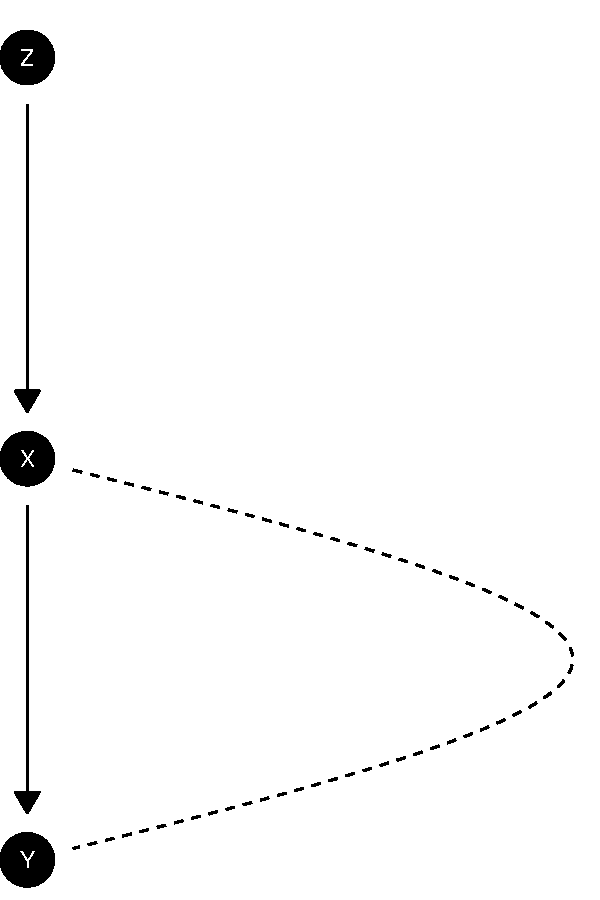
\includegraphics[width=0.6\textwidth,height=\textheight]{paper_files/figure-pdf/fig-plots-1.pdf}

}

\subcaption{\label{fig-plots-1}Without options}

\end{minipage}%
%
\begin{minipage}{0.50\linewidth}

\centering{

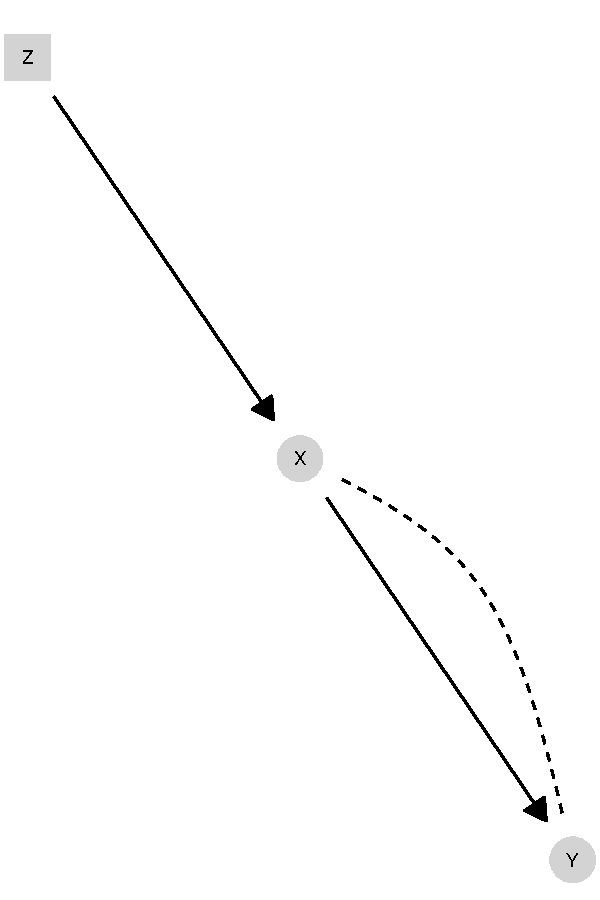
\includegraphics[width=0.6\textwidth,height=\textheight]{paper_files/figure-pdf/fig-plots-2.pdf}

}

\subcaption{\label{fig-plots-2}With options}

\end{minipage}%

\caption{\label{fig-plots}Examples of model graphs.}

\end{figure}%

\subsection{Model inspection}\label{model-inspection}

When a model is defined, \texttt{CausalQueries} generates a set of
internal objects that are used for all inferential tasks. These include
default parameter values and default priors, as well as matrices that
map from parameters to causal types, and from causal types to data
types. These objects generally do not need to be examined by the users,
however \texttt{CausalQueries} provides a pair of functions,
\texttt{inspect()} and \texttt{grab()}, that lets users quickly examine
these elements

Table~\ref{tbl-core} summarizes features of a causal model that can be
examined using \texttt{inspect()}.

\begin{longtable}[]{@{}
  >{\raggedright\arraybackslash}p{(\columnwidth - 2\tabcolsep) * \real{0.4000}}
  >{\raggedright\arraybackslash}p{(\columnwidth - 2\tabcolsep) * \real{0.6000}}@{}}
\caption{Elements of a model that can be inspected using
\texttt{inspect()}.}\label{tbl-core}\tabularnewline
\toprule\noalign{}
\begin{minipage}[b]{\linewidth}\raggedright
Element
\end{minipage} & \begin{minipage}[b]{\linewidth}\raggedright
Description
\end{minipage} \\
\midrule\noalign{}
\endfirsthead
\toprule\noalign{}
\begin{minipage}[b]{\linewidth}\raggedright
Element
\end{minipage} & \begin{minipage}[b]{\linewidth}\raggedright
Description
\end{minipage} \\
\midrule\noalign{}
\endhead
\bottomrule\noalign{}
\endlastfoot
\texttt{statement} & A character string describing causal relations
using dagitty syntax. \\
\texttt{nodes} & A list containing the nodes in the model. \\
\texttt{parents\_df} & A table listing nodes, whether they are root
nodes or not, and the number and names of parents they have. \\
\texttt{parameters} & A vector of `true' parameters. \\
\texttt{parameter\_names} & A vector of names of parameters. \\
\texttt{parameter\_mapping} & A matrix mapping from parameters into data
types. \\
\texttt{parameter\_matrix} & A matrix mapping from parameters into
causal types. \\
\texttt{parameters\_df} & A data frame containing parameter
information. \\
\texttt{causal\_types} & A data frame listing causal types and the nodal
types that produce them. \\
\texttt{nodal\_types} & A list with the nodal types of the model. \\
\texttt{data\_types} & A list with all data types consistent with the
model; for options see \texttt{?get\_all\_data\_types}. \\
\texttt{ambiguities\_matrix} & A matrix mapping from causal types into
data types. \\
\texttt{type\_prior} & A matrix of type probabilities using priors. \\
\texttt{prior\_hyperparameters} & A vector of alpha values used to
parameterize Dirichlet prior distributions; optionally provide node
names to reduce output, e.g.,
\texttt{inspect(prior\_hyperparameters,\ nodes\ =\ c(\textquotesingle{}M\textquotesingle{},\ \textquotesingle{}Y\textquotesingle{}))}. \\
\texttt{prior\_event\_probabilities} & A vector of data (event)
probabilities given a single realization of parameters; for options see
\texttt{?get\_event\_probabilities}. \\
\texttt{prior\_distribution} & A data frame of the parameter prior
distribution. \\
\texttt{posterior\_distribution} & A data frame of the parameter
posterior distribution. \\
\texttt{posterior\_event\_probabilities} & A sample of data (event)
probabilities from the posterior. \\
\texttt{type\_distribution} & A matrix of type probabilities using
posteriors. \\
\texttt{data} & A data frame with data that was provided to update the
model. \\
\texttt{stanfit} & A \texttt{stanfit} object generated by Stan; prints
\texttt{stanfit} summary with updated parameter names. \\
\texttt{stan\_summary} & A list of Stan outputs that includes
\texttt{stanfit}, \texttt{data}, and, if requested when updating the
model, posterior \texttt{event\_probabilities} and
\texttt{type\_distribution}; prints \texttt{stanfit} summary with
updated parameter names. \\
\end{longtable}

\subsection{Tailoring models}\label{tailoring-models}

When a causal statement is provided to \texttt{make\_model()}, a model
is formed with a set of default assumptions: in particular, no
restrictions are placed on nodal types and flat priors are assumed over
all parameters. These features can be adjusted after a model is formed
using \texttt{set\_confounds}, \texttt{set\_restrictions},
\texttt{set\_priors}, and \texttt{set\_parameters}.

\subsubsection{Allowing confounding}\label{sec-confounding}

Unobserved confounding between two (or more) nodes arises when the nodal
types for the nodes are not independent. For instance, in the
\(X \rightarrow Y\) graph, there are \(2\) nodal types for \(X\) and
\(4\) for \(Y\). There are thus \(8\) joint nodal types (or causal
types), as shown in Table~\ref{tbl-joint}.

\begin{longtable}[]{@{}
  >{\centering\arraybackslash}p{(\columnwidth - 6\tabcolsep) * \real{0.2500}}
  >{\centering\arraybackslash}p{(\columnwidth - 6\tabcolsep) * \real{0.2500}}
  >{\centering\arraybackslash}p{(\columnwidth - 6\tabcolsep) * \real{0.2500}}
  >{\centering\arraybackslash}p{(\columnwidth - 6\tabcolsep) * \real{0.2500}}@{}}
\caption{Nodal types in \(X \rightarrow Y\)
model.}\label{tbl-joint}\tabularnewline
\toprule\noalign{}
\begin{minipage}[b]{\linewidth}\centering
\end{minipage} & \begin{minipage}[b]{\linewidth}\centering
\(\theta^X_{0}\)
\end{minipage} & \begin{minipage}[b]{\linewidth}\centering
\(\theta^X_{1}\)
\end{minipage} & \begin{minipage}[b]{\linewidth}\centering
\(\sum\)
\end{minipage} \\
\midrule\noalign{}
\endfirsthead
\toprule\noalign{}
\begin{minipage}[b]{\linewidth}\centering
\end{minipage} & \begin{minipage}[b]{\linewidth}\centering
\(\theta^X_{0}\)
\end{minipage} & \begin{minipage}[b]{\linewidth}\centering
\(\theta^X_{1}\)
\end{minipage} & \begin{minipage}[b]{\linewidth}\centering
\(\sum\)
\end{minipage} \\
\midrule\noalign{}
\endhead
\bottomrule\noalign{}
\endlastfoot
\(\theta^Y_{00}\) & \(\Pr(\theta^X_0, \theta^Y_{00})\) &
\(\Pr(\theta^X_1, \theta^Y_{00})\) & \(\Pr(\theta^Y_{00})\) \\
\(\theta^Y_{10}\) & \(\Pr(\theta^X_0, \theta^Y_{10})\) &
\(\Pr(\theta^X_1, \theta^Y_{10})\) & \(\Pr(\theta^Y_{10})\) \\
\(\theta^Y_{01}\) & \(\Pr(\theta^X_0, \theta^Y_{01})\) &
\(\Pr(\theta^X_1, \theta^Y_{01})\) & \(\Pr(\theta^Y_{01})\) \\
\(\theta^Y_{11}\) & \(\Pr(\theta^X_0, \theta^Y_{11})\) &
\(\Pr(\theta^X_1, \theta^Y_{11})\) & \(\Pr(\theta^Y_{11})\) \\
\(\sum\) & \(\Pr(\theta^X_0)\) & \(\Pr(\theta^X_1)\) & 1 \\
\end{longtable}

Table~\ref{tbl-joint} has eight interior elements so that an
unconstrained joint distribution would have seven degrees of freedom. A
no-confounding assumption means that
\(\Pr(\theta^X, \theta^Y) = \Pr(\theta^X)\Pr(\theta^Y)\). In this case,
it is sufficient to put a distribution on the marginals, and there would
be \(3\) degrees of freedom for \(Y\) and \(1\) for \(X\), totaling
\(4\) rather than \(7\).

To allow for an unconstrained joint distribution the parameters data
frame for this model would have two parameter families for parameters
associated with the node \(Y\). Each family captures the conditional
distribution of \(Y\)'s nodal types, given \(X\). For instance the
parameter \texttt{Y01\_X.1} can be interpreted as
\(\Pr(\theta^Y = \theta^Y_{01} | \theta^X=1)\). See again
Table~\ref{tbl-lipidspar} for an example of a parameter matrix with
confounding.

The confounding structure can affect the number of parameters given the
underlying DAG. Table~\ref{tbl-dof} illustrates the number of
independent parameters required given different types of confounding.

\begin{longtable}[]{@{}lc@{}}

\caption{\label{tbl-dof}Number of different independent parameters
(degrees of freedom) for different three-node models.}

\tabularnewline

\toprule\noalign{}
Model & Degrees of freedom \\
\midrule\noalign{}
\endhead
\bottomrule\noalign{}
\endlastfoot
\texttt{X\ -\textgreater{}\ Y\ \textless{}-\ W} & 17 \\
\texttt{X\ -\textgreater{}\ Y\ \textless{}-\ W;\ X\ \textless{}-\textgreater{}\ W}
& 18 \\
\texttt{X\ -\textgreater{}\ Y\ \textless{}-\ W;\ X\ \textless{}-\textgreater{}\ Y;\ W\ \textless{}-\textgreater{}\ Y}
& 62 \\
\texttt{X\ -\textgreater{}\ Y\ \textless{}-\ W;\ X\ \textless{}-\textgreater{}\ Y;\ W\ \textless{}-\textgreater{}\ Y;\ X\ \textless{}-\textgreater{}\ W}
& 63 \\
\texttt{X\ -\textgreater{}\ W\ -\textgreater{}\ Y\ \textless{}-\ X} &
19 \\
\texttt{X\ -\textgreater{}\ W\ -\textgreater{}\ Y\ \textless{}-\ X;\ W\ \textless{}-\textgreater{}\ Y}
& 64 \\
\texttt{X\ -\textgreater{}\ W\ -\textgreater{}\ Y\ \textless{}-\ X;\ X\ \textless{}-\textgreater{}\ W;\ W\ \textless{}-\textgreater{}\ Y}
& 67 \\
\texttt{X\ -\textgreater{}\ W\ -\textgreater{}\ Y\ \textless{}-\ X;\ X\ \textless{}-\textgreater{}\ W;\ W\ \textless{}-\textgreater{}\ Y;\ X\ \textless{}-\textgreater{}\ Y}
& 127 \\

\end{longtable}

\subsubsection{Setting restrictions}\label{restrictions}

Sometimes it is helpful to constrain the set of types. In
\texttt{CausalQueries} this is done at the level of nodal types, with
restrictions on causal types following restrictions on nodal types.

To illustrate, in analyses of data with imperfect compliance, as in our
Lipids model example, it is common to impose a monotonicity assumption:
that \(X\) does not respond negatively to \(Z\). This is one of the
conditions needed to interpret instrumental variables estimates as
(consistent) estimates of the complier average treatment effect. In
\texttt{CausalQueries} we can impose this assumption as follows:

\begin{verbatim}
R> model_restricted <- 
+  lipids_model |> 
+  set_restrictions("X[Z=1] < X[Z=0]")
\end{verbatim}

In words: we restrict the model by removing types for which \(X\)
decreases in \(Z\). If we wanted to retain only this nodal type rather
than remove it, we could do so by passing \texttt{keep\ =\ TRUE} as an
argument to the \texttt{set\_restrictions()} function call. Users can
use \texttt{inspect(model,\ "parameter\_matrix")} to view the resulting
parameter matrix in which both the set of parameters and the set of
causal types are restricted.

Restrictions in \texttt{CausalQueries} can be set in many other ways:

\begin{itemize}
\item
  Using nodal type labels:

\begin{verbatim}
R> model <- 
+  lipids_model |>
+  set_restrictions(labels = list(X = "01", Y = c("00", "01", "11")), 
+                   keep = TRUE)
\end{verbatim}
\item
  Using wildcards in nodal type labels:

\begin{verbatim}
R> model <- lipids_model |>
+  set_restrictions(labels = list(Y = "?0"))
\end{verbatim}
\item
  In models with confounding, restrictions can be added to nodal types
  conditional on the values of other nodal types using a \texttt{given}
  argument:

\begin{verbatim}
R> model <- lipids_model |>
+  set_restrictions(labels = list(Y = c('00', '11')), given = 'X.00')
\end{verbatim}
\end{itemize}

Setting restrictions sometimes involves using causal syntax (see
Section~\ref{sec-syntax} for a guide to the syntax used by
\texttt{CausalQueries}). The help file in \texttt{?set\_restrictions}
provides further details and examples of restrictions users can set.

\subsubsection{Setting Priors}\label{priors}

Priors on model parameters can be added to the parameters data frame and
interpreted as alpha parameters of a Dirichlet distribution. The
Dirichlet distribution is a probability distribution over an \(n-1\)
dimensional unit simplex. It can be considered a generalization of the
Beta distribution and is parametrized by an \(n\)-dimensional positive
vector \(\alpha\). Thus, for example a Dirichlet with
\(\alpha = (1, 1, 1, 1, 1)\) gives a probability distribution over all
non-negative \(5\)-dimensional vectors that sum to \(1\),
e.g.~\((0.1, 0.1, 0.1, 0.1, 0.6)\) or \((0.1, 0.2, 0.3, 0.3, 0.1)\).
This particular value for \(\alpha\) implies that all such vectors are
equally likely. Other values for \(\alpha\) can be used to control the
expectation and certainty for each dimension. For instance, the vector
\(\alpha = (100, 1, 1, 1, 100)\) would result in more weight on
distributions that are close to \((0.5, 0, 0, 0, 0.5)\).

In \texttt{CausalQueries}, priors are generally specified over the
distribution of nodal types.\footnote{If there is confounding in the
  model, priors are specified over the conditional distribution of nodal
  types.} For instance, in a model represented by \(X \rightarrow Y\),
we have one Dirichlet distribution over the two types for \(\theta^X\)
and one Dirichlet distribution over the four types for \(\theta^Y\).

Importantly, it is implicitly assumed that priors are independent across
families. Thus, for instance, in a model represented by
\(X \rightarrow Y\), we specify beliefs over \(\lambda^X\) and over
\(\lambda^Y\) separately. \texttt{CausalQueries} does not let users
specify correlated beliefs over these parameters.\footnote{Users can
  specify beliefs about \(\lambda^Y\) given \(\theta^X\) if a model
  involves possible confounding. But this statement is about beliefs
  over a joint distribution, not jointly distributed beliefs.}

Prior hyperparameters are set to unity by default, corresponding to
uniform priors. Users can retrieve the model's priors as follows:

\begin{verbatim}
R> lipids_model |> 
+  inspect("prior_hyperparameters", nodes = "X") 
\end{verbatim}

\begin{verbatim}
#> 
#> Alpha parameter values used for Dirichlet prior distributions:
#> 
#> X.00 X.10 X.01 X.11 
#>    1    1    1    1
\end{verbatim}

Alternatively users can set Jeffreys priors using \texttt{set\_priors()}
as follows:

\begin{verbatim}
R> model <- lipids_model |> 
+  set_priors(distribution = "jeffreys")
\end{verbatim}

Users can also provide custom priors. The simplest way to specify custom
priors is to add them as a vector of numbers using
\texttt{set\_priors()}. For instance:

\begin{verbatim}
R> lipids_model |> 
+  set_priors(node = "X", alphas = 1:4) |> 
+  inspect("prior_hyperparameters", nodes = "X")
\end{verbatim}

\begin{verbatim}
#> 
#> Alpha parameter values used for Dirichlet prior distributions:
#> 
#> X.00 X.10 X.01 X.11 
#>    1    2    3    4
\end{verbatim}

The priors here should be interpreted as indicating
\(\alpha_X = (1,2, 3, 4)\), which implies a distribution over
\((\lambda^X_{00},\lambda^X_{10}, \lambda^X_{01}, \lambda^X_{11})\) with
expectation
\(\left(\frac1{10}, \frac2{10}, \frac3{10}, \frac4{10} \right)\).

Providing priors as a vector of numbers for larger models can be hard.
For that reason, \texttt{set\_priors()} allows for more targeted
modifications of the parameter vector. For instance:

\begin{verbatim}
R> lipids_model |>
+  set_priors(statement = "X[Z=1] > X[Z=0]", alphas = 3) |>
+  inspect("prior_hyperparameters", nodes = "X")
\end{verbatim}

\begin{verbatim}
#> 
#> Alpha parameter values used for Dirichlet prior distributions:
#> 
#> X.00 X.10 X.01 X.11 
#>    1    1    3    1
\end{verbatim}

Setting priors requires mapping alpha values to parameters, and so the
problem of altering priors reduces to selecting rows of the
\texttt{parameters\_df} data frame at which to alter values. When
specifying a causal statement as above, \texttt{CausalQueries}
internally identifies nodal types consistent with the statement, which
identifies parameters to alter priors for.

We can achieve the same result as above by specifying nodal types for
which we would like to adjust the priors. \texttt{set\_priors()} allows
for the specification of any non-redundant combination of arguments on
the \texttt{param\_names}, \texttt{node}, \texttt{nodal\_type},
\texttt{param\_set}, and \texttt{given} columns of
\texttt{parameters\_df} to identify parameters to set priors for
uniquely. Alternatively, a fully formed subsetting statement may be
supplied to \texttt{alter\_at}. Since all these arguments are mapped to
the parameters they identify internally, they may be used
interchangeably.\footnote{See \texttt{?set\_priors} and
  \texttt{?make\_priors} for many more examples.}

While highly targeted prior setting is convenient and flexible, it
should be used cautiously. Setting priors on specific parameters in
complex models, especially models involving confounding, may strongly
affect inferences. Furthermore, note that flat priors over nodal types
do not necessarily translate into flat priors over queries. Flat priors
over parameters in a parameter family put equal weight on each nodal
type, which can translate into strong assumptions on causal quantities
of interest. For instance, in an \(X \rightarrow Y\) model in which
negative effects are ruled out, the average causal effect implied by
flat priors is \(1/3\). This can be seen by querying the model as
follows:

\begin{verbatim}
R> query <- 
+  make_model("X -> Y") |>
+  set_restrictions(decreasing("X", "Y")) |>
+  query_model("Y[X=1] - Y[X=0]", using = "priors")
\end{verbatim}

More subtly, the \emph{structure} of a model, coupled with flat priors,
has substantive importance for priors on causal quantities. For
instance, with flat priors, prior on the probability that \(X\) has a
positive effect on \(Y\) in the model \(X \rightarrow Y\) is centered on
\(1/4\). But prior on the probability that \(X\) positively affects
\(Y\) in the model \(X \rightarrow M \rightarrow Y\) is centered on
\(1/8\).

Caution regarding priors is essential when models are not identified, as
is the case for many models considered here. For some quantities, the
marginal posterior distribution reflects the marginal prior distribution
\citep{poirier_revising_1998}.

\subsubsection{Setting Parameters}\label{parameters}

By default, models have a vector of parameter values included in the
\texttt{parameters\_df} data frame. These are useful for generating data
or for situations, such as process tracing, when one wants to make
inferences about causal types (\(\theta\)), given case-level data, under
the assumption that the model is known.

The logic for setting parameters is similar to that for setting priors.
The critical difference is that whereas the \(\alpha\) value placed on
nodal types can be any positive number---capturing our certainty over
the parameter value---the parameter values must lie in the unit
interval, \([0,1]\). If passed parameter values do not lie in the unit
interval, they are normalized so that they do.

The causal model below has two parameter sets, one for \(X\) and one for
\(Y\), with two nodal types for \(X\) and four for \(Y\). The key
feature of the parameters is that they must sum to \(1\) within each
parameter set.

\begin{verbatim}
R> make_model("X -> Y") |> 
+  inspect("parameters")
\end{verbatim}

\begin{verbatim}
#> 
#> Model parameters with associated probabilities: 
#> 
#>  X.0  X.1 Y.00 Y.10 Y.01 Y.11 
#> 0.50 0.50 0.25 0.25 0.25 0.25
\end{verbatim}

The example below illustrates a change in the value of the parameter
that corresponds to a positive effect of \(X\) on \(Y\). Here, the nodal
type \texttt{Y.Y01} is set to be \(0.7\), while the other nodal types of
this parameter set were re-normalized so that the parameters in the set
still sum up to one.

\begin{verbatim}
R> make_model("X -> Y") |>
+  set_parameters(statement = "Y[X=1] > Y[X=0]", parameters = .7) |>
+  inspect("parameters")
\end{verbatim}

\begin{verbatim}
#> 
#> Model parameters with associated probabilities: 
#> 
#>  X.0  X.1 Y.00 Y.10 Y.01 Y.11 
#>  0.5  0.5  0.1  0.1  0.7  0.1
\end{verbatim}

\subsection{Drawing and manipulating
data}\label{drawing-and-manipulating-data}

Once a model has been defined, it is possible to simulate data from the
model using the \texttt{make\_data()} function. For instance, this can
be useful for assessing a model's expected performance given data drawn
from some speculated set of parameter values.

\subsubsection{Drawing data basics}\label{drawing-data-basics}

Generating data requires a specification of parameter values. The
parameter values in the parameters dataframe are used by default.
Otherwise users can provide parameters on the fly.

\begin{verbatim}
R> sample_data_1 <- 
+  lipids_model |> 
+  make_data(n = 4)
\end{verbatim}

However, users can also specify parameters directly or draw parameters
from a prior or posterior distribution. For instance:

\begin{verbatim}
R> lipids_model |>
+  make_data(n = 3, param_type = "prior_draw")
\end{verbatim}

\begin{verbatim}
#>   Z X Y
#> 1 0 1 0
#> 2 1 1 0
#> 3 1 1 1
\end{verbatim}

The resulting data is ordered by data type, as shown in the example
above.

\subsubsection{Drawing incomplete data}\label{drawing-incomplete-data}

\texttt{CausalQueries} can be used when researchers have gathered
different amounts of data for different nodes. For instance, a
researcher could collect data on \(X\) and \(Y\) for all units, but data
on \(M\) only for some. The function \texttt{make\_data()} allows users
to draw data like this if they specify a data strategy indicating the
probabilities of observing data on different nodes, possibly as a
function of prior nodes observed.

\begin{verbatim}
R> sample_data_2 <-
+  lipids_model |>
+  make_data(n = 8,
+            nodes = list(c("Z", "Y"), "X"),
+            probs = list(1, .5),
+            subsets = list(TRUE, "Z==1 & Y==0"))
\end{verbatim}

\begin{verbatim}
#> # A tibble: 2 x 5
#>   node_names nodes     n_steps probs subsets    
#>   <chr>      <list>    <lgl>   <dbl> <chr>      
#> 1 Z, Y       <chr [2]> NA        1   TRUE       
#> 2 X          <chr [1]> NA        0.5 Z==1 & Y==0
\end{verbatim}

\begin{verbatim}
R> sample_data_2
\end{verbatim}

\begin{verbatim}
#>   Z  X Y
#> 1 0 NA 0
#> 2 0 NA 1
#> 3 0 NA 1
#> 4 0 NA 1
#> 5 0 NA 1
#> 6 0 NA 1
#> 7 1 NA 1
#> 8 1 NA 1
\end{verbatim}

\subsubsection{Reshaping data}\label{reshaping-data}

Whereas data usually comes in ``long form'', with one row per
observation, the data passed to Stan during model updating is in a
``compact'' form. The latter records only the number of units of each
data type, grouped by data ``strategy''---an indicator of the nodes for
which researchers gathered data. \texttt{CausalQueries} includes
functions that let users move between these two forms.

\begin{verbatim}
R> sample_data_2 |> 
+  collapse_data(lipids_model)
\end{verbatim}

\begin{verbatim}
#>   event strategy count
#> 1  Z0Y0       ZY     1
#> 2  Z1Y0       ZY     0
#> 3  Z0Y1       ZY     5
#> 4  Z1Y1       ZY     2
\end{verbatim}

In the same way, it is possible to move from compact to long data using
\texttt{expand\_data()}. Note that \texttt{NA}'s are interpreted as data
not being sought.

\section{Updating models}\label{sec-update}

The approach used by the \texttt{CausalQueries} package to update
parameter values given observed data relies on the Stan programming
language \citep{carpenter_stan_2017}. Below we explain the data required
by the generic Stan program implemented in the package, the structure of
that program, and then show how to use the package to produce posterior
draws of parameters.

\subsection{Data for Stan}\label{data-for-stan}

We use a generic Stan program that works for all binary causal models.
The main advantage of the generic program is that it allows us to pass
the details of the causal model as data inputs to Stan instead of
generating individual Stan programs for each causal model.
\hyperref[sec-stancode]{Appendix B} provides the complete Stan model
code.

The data required by the Stan program includes vectors of observed data
and priors on parameters, as well as a set of matrices needed for the
mapping between events, data types, causal types, and parameters. In
addition, data passed to \texttt{stan} includes counts of all relevant
quantities as well as start and end positions of parameters pertaining
to specific nodes and distinct data strategies.

The internal function \texttt{prep\_stan\_data()} takes the model and
data as arguments and produces a list with all objects that are required
by the generic Stan program. Package users do not need to call the
\texttt{prep\_stan\_data()} function directly.

\subsection{How the Stan program
works}\label{how-the-stan-program-works}

The Stan model involves the following elements: (1) a specification of
priors over sets of parameters, (2) a mapping from parameters to event
probabilities, and (3) a likelihood function. Below, we describe each of
those elements in more detail.

\subsubsection{Probability distributions over parameter
sets}\label{probability-distributions-over-parameter-sets}

The causal structure provided by a DAG allows us to reduce the problem
of generating a probability distribution over all parameters to one of
generating distributions over ``sets'' of parameters. Without unobserved
confounding, these sets correspond to the nodal types for each node: we
have a probability distribution over the set of nodal types.

Thus for instance we have two parameter sets in the \(X \rightarrow Y\)
model. We have a \(2\)-dimensional Dirichlet distribution over the \(X\)
nodal types,
\((\lambda^X_0, \lambda^X_1) \sim Dirichlet(\alpha^X_0, \alpha^X_1).\) ,
and a \(4\)-dimensional Dirichlet over the \(Y\) nodal types,
\((\lambda^Y_{00}, \lambda^Y_{10}, \lambda^Y_{01}, \lambda^Y_{11}) \sim Dirichlet(\alpha^Y_{00}, \alpha^Y_{10}, \alpha^Y_{01}, \alpha^Y_{11}).\)

In cases with confounding, these are sets of nodal types for a given
node \emph{given} values of other nodes.

\subsubsection{Event probabilities}\label{event-probabilities}

We calculate the probability of data types for any candidate parameter
vector \(\lambda\). This is done using a matrix that maps from
parameters into data types.

In cases without confounding, there is a column for each data type; the
matrix indicates which nodes in each set ``contribute'' to the data
type, and the probability of the data type is found by summing within
sets and taking the product over sets. To illustrate, we can examine the
parameter mapping matrix for a simple model using the \texttt{inspect()}
function as follows:

\begin{verbatim}
R> make_model("X -> Y") |> 
+  inspect("parameter_mapping") 
\end{verbatim}

\begin{verbatim}
#> 
#> Parameter mapping matrix: 
#> 
#>   Maps from parameters to data types, with
#>   possibly multiple columns for each data type
#>   in cases with confounding. 
#> 
#>      X0Y0 X1Y0 X0Y1 X1Y1
#> X.0     1    0    1    0
#> X.1     0    1    0    1
#> Y.00    1    1    0    0
#> Y.10    0    1    1    0
#> Y.01    1    0    0    1
#> Y.11    0    0    1    1
\end{verbatim}

In this model, the probability of data type \texttt{X0Y0}, \(w_{00}\) is
\(\lambda^X_0\times \lambda^Y_{00} + \lambda^X_0\times \lambda^Y_{01}\).
This formula can be read from the parameter mapping matrix by combining
a parameter vector with the first column of the matrix, taking the
product of the probability of \texttt{X.0} and the \emph{sum} of the
probabilities for \texttt{Y.00} and \texttt{Y.01}.

In cases with confounding, the approach is similar, except that the
parameter mapping matrix can contain multiple columns for each data type
to capture non-independence between nodes.

In the case of incomplete data, we first identify the set of data
strategies, where a collection of a data strategy might be of the form
``gather data on \(X\) and \(M\), but not \(Y\), for \(n_1\) cases and
gather data on \(X\) and \(Y\), but not \(M\), for \(n_2\) cases.''
Within a data strategy, the probability of an observed event is given by
summing the probabilities of the types that could give rise to a
particular pattern of incomplete data.

\subsubsection{Data probability}\label{data-probability}

Once we have the event probabilities in hand for each data strategy, we
are ready to calculate the probability of the data. For a given data
strategy, this is given by a multinomial distribution with these event
probabilities. When there is incomplete data, and so there are multiple
data strategies, the probability of the data is given by the product of
the multinomial probabilities for data generated by each strategy.

\subsection{Implementation}\label{implementation}

The function \texttt{update\_model(model,\ data)} is used to update a
model, that is, append a posterior distribution over model parameters to
the model. The \texttt{data} argument provides a data frame containing
some or all of the nodes in the model. The function
\texttt{update\_model()} relies on \texttt{rstan::sampling()} to draw
from the posterior distribution, and one can pass any additional
arguments accepted by \texttt{rstan::sampling()}. Given that model
updating can sometimes be slow for complex models, we show in
\hyperref[sec-parallel]{Appendix A} how users can utilize
parallelization to improve computation speed.
\hyperref[sec-benchmark]{Appendix C} provides an overview of model
updating benchmarks, evaluating the effects of model complexity and data
size on updating times.

Note that if no data is passed to \texttt{update\_model()} the Stan
model is still implemented and the posterior distribution appended to
the model can be interpreted as draws from the prior distribution.

\subsection{Incomplete and censored
data}\label{incomplete-and-censored-data}

\texttt{CausalQueries} assumes that missing data is missing at random,
conditional on observed data. For instance, in an
\(X \rightarrow M \rightarrow Y\) model, a researcher might have chosen
to collect data on \(M\) in a random set of cases in which \(X=1\) and
\(Y=1\). If there are positive relations at each stage, one may be more
likely to observe \(M\) in cases in which \(M=1\). However, the
observation of \(M\) is still random and conditional on the observed
\(X\) and \(Y\) data. The Stan model in \texttt{CausalQueries} takes
account of this kind of sampling by assessing the probability of
observing a particular pattern of data within each data
strategy.\footnote{For further discussion, see Section 9.2.3.2 in
  \citet{humphreys_integrated_2023}.}

In addition, it is possible to indicate when data has been censored and
for the Stan model to take this into account also. For instance,
consider a situation in which we only observe \(X\) in cases when
\(X=1\) and not when \(X=0\). This kind of sampling is non-random and
conditional on observables. It can be taken into account, however, by
indicating to Stan that the probability of observing a particular data
type is \(0\), regardless of parameter values. This can done using the
\texttt{censored\_types} argument in \texttt{update\_model()}.

To illustrate, in the example below, we observe perfectly correlated
data for \(X\) and \(Y\). If we are aware that data in which
\(X \neq Y\) has been censored, then when we update, we do not move
towards a belief that \(X\) causes \(Y\).

\begin{verbatim}
R> data <- data.frame(X = rep(0:1, 5), Y = rep(0:1, 5))
R> 
R> list(
+  uncensored = 
+    update_model(make_model("X -> Y"),
+                 data),
+  censored = 
+    update_model(make_model("X -> Y"), 
+                 data, 
+                 censored_types = c("X1Y0",  "X0Y1"))
+  ) |>
+  query_model("Y[X=1] - Y[X=0]", using = "posteriors") |> 
+  subset(select = c("model", "query", "mean", "sd"))
\end{verbatim}

\begin{verbatim}
#> 
#> Causal queries generated by query_model
#> 
#> |model      |query           |  mean|    sd|
#> |:----------|:---------------|-----:|-----:|
#> |uncensored |Y[X=1] - Y[X=0] | 0.597| 0.193|
#> |censored   |Y[X=1] - Y[X=0] | 0.014| 0.319|
\end{verbatim}

\subsection{Output}\label{output}

The primary output from \texttt{update\_model()} is a model with an
attached posterior distribution over model parameters stored as a data
frame in the model list. This posterior distribution can be directly
accessed using the \texttt{inspect()} function as follows:

\begin{verbatim}
R> model <-
+  make_model("X -> Y")  |> 
+  update_model()
R> 
R> posterior <- grab(model, "posterior_distribution")  
\end{verbatim}

In addition, a distribution of causal types is stored by default; the
\texttt{stanfit} object and a distribution over event probabilities are
optionally saved as follows:

\begin{verbatim}
R> lipids_model <- 
+  lipids_model |> 
+  update_model(keep_fit = TRUE,
+               keep_event_probabilities = TRUE)
\end{verbatim}

The summary of the Stan model can be accessed using \texttt{inspect()}
function and is saved in the updated model object by default. This
provides two measures to help assess convergence.

\begin{verbatim}
R> make_model("X -> Y")  |> 
+  update_model(keep_type_distribution = FALSE) |>
+  inspect("stan_summary") 
\end{verbatim}

\begin{verbatim}
#> 
#> Stan model summary:
#> 
#> Inference for Stan model: simplexes.
#> 4 chains, each with iter=2000; warmup=1000; thin=1; 
#> post-warmup draws per chain=1000, total post-warmup draws=4000.
#> 
#>             mean se_mean   sd   2.5%   25%   50%   75% 97.5% n_eff Rhat
#> X.0         0.51    0.01 0.29   0.03  0.26  0.51  0.76  0.98  2978    1
#> X.1         0.49    0.01 0.29   0.02  0.24  0.49  0.74  0.97  2978    1
#> Y.00        0.25    0.00 0.19   0.01  0.10  0.21  0.37  0.71  2114    1
#> Y.10        0.25    0.00 0.19   0.01  0.09  0.21  0.37  0.71  4401    1
#> Y.01        0.25    0.00 0.20   0.01  0.09  0.21  0.37  0.72  4105    1
#> Y.11        0.25    0.00 0.19   0.01  0.09  0.21  0.37  0.70  4114    1
#> lp__       -7.53    0.04 1.60 -11.41 -8.40 -7.17 -6.34 -5.43  1363    1
#> 
#> Samples were drawn using NUTS(diag_e) at Mon Oct 21 18:16:50 2024.
#> For each parameter, n_eff is a crude measure of effective sample size,
#> and Rhat is the potential scale reduction factor on split chains (at 
#> convergence, Rhat=1).
\end{verbatim}

This summary provides information on the distribution of parameters and
convergence diagnostics, summarized in the \texttt{Rhat} column. The
last row shows the unnormalized log density on Stan's unconstrained
space, which is intended to diagnose sampling efficiency and evaluate
approximations.\footnote{See
  \href{https://mc-stan.org/cmdstanr/reference/fit-method-lp.html}{Stan
  documentation} for more details.} This summary can also include
summaries for the transformed parameters if users retain
these.\footnote{See \textbf{?@tbl-additional} for options.}

If users wish to run more advanced diagnostics of performance, they can
retain and access the ``raw'' Stan output as follows:

\begin{verbatim}
R> model <- 
+  make_model("X -> Y") |> 
+  update_model(refresh = 0, keep_fit = TRUE)
\end{verbatim}

Note that the raw output uses labels from the generic Stan model:
\texttt{lambda} for the vector of parameters, corresponding to the
parameters in the parameters data frame
(\texttt{inspect(model,\ "parameters\_df")}), a vector \texttt{types}
for the causal types (\texttt{inspect(model,\ "causal\_types")}) and
\texttt{event\_probabilities} for the event probabilities
(\texttt{inspect(model,\ "event\_probabilities")}).

\begin{verbatim}
R> model |> 
+  inspect("stanfit")
\end{verbatim}

\begin{verbatim}
#> 
#> Stan model summary:
#> Inference for Stan model: simplexes.
#> 4 chains, each with iter=2000; warmup=1000; thin=1; 
#> post-warmup draws per chain=1000, total post-warmup draws=4000.
#> 
#>             mean se_mean   sd   2.5%   25%   50%   75% 97.5% n_eff Rhat
#> lambdas[1]  0.51    0.01 0.30   0.02  0.24  0.51  0.78  0.98  3346    1
#> lambdas[2]  0.49    0.01 0.30   0.02  0.22  0.49  0.76  0.98  3346    1
#> lambdas[3]  0.25    0.00 0.19   0.01  0.09  0.20  0.36  0.72  1960    1
#> lambdas[4]  0.25    0.00 0.19   0.01  0.10  0.21  0.37  0.69  4566    1
#> lambdas[5]  0.25    0.00 0.19   0.01  0.09  0.22  0.37  0.69  4144    1
#> lambdas[6]  0.25    0.00 0.19   0.01  0.09  0.21  0.37  0.72  4266    1
#> types[1]    0.12    0.00 0.13   0.00  0.03  0.07  0.17  0.50  2464    1
#> types[2]    0.12    0.00 0.14   0.00  0.02  0.07  0.17  0.50  2187    1
#> types[3]    0.13    0.00 0.14   0.00  0.03  0.08  0.19  0.50  3659    1
#> types[4]    0.12    0.00 0.13   0.00  0.03  0.08  0.17  0.49  3782    1
#> types[5]    0.13    0.00 0.14   0.00  0.03  0.08  0.18  0.51  3546    1
#> types[6]    0.12    0.00 0.13   0.00  0.02  0.08  0.18  0.49  3390    1
#> types[7]    0.13    0.00 0.14   0.00  0.02  0.08  0.18  0.51  3555    1
#> types[8]    0.12    0.00 0.13   0.00  0.02  0.08  0.18  0.48  4074    1
#> lp__       -7.59    0.05 1.67 -11.78 -8.39 -7.24 -6.36 -5.46  1100    1
#> 
#> Samples were drawn using NUTS(diag_e) at Mon Oct 21 18:16:56 2024.
#> For each parameter, n_eff is a crude measure of effective sample size,
#> and Rhat is the potential scale reduction factor on split chains (at 
#> convergence, Rhat=1).
\end{verbatim}

Users can then pass the Stan fit object to other diagnostic packages
such as \texttt{bayesplot}.

\section{Queries}\label{sec-query}

\texttt{CausalQueries} provides functionality to pose and answer
elaborate causal queries. The key approach is to code causal queries as
functions of causal types and return a distribution over the queries
implied by the distribution over causal types.

\subsection{Calculating factual and counterfactual
quantities}\label{sec-propagation}

An essential step in calculating most queries is assessing what outcomes
will arise for causal types given different interventions on nodes. In
practice, we map from causal types to data types by propagating realized
values on nodes forward in the DAG, moving from exogenous or intervened
upon nodes to their descendants in generational order. An internal
function, \texttt{realise\_outcomes()}, achieves this by traversing the
DAG while recording the values implied by realizations on the node's
parents for each node's nodal types.

To illustrate, consider the first causal type of a \(X \rightarrow Y\)
model:

\begin{enumerate}
\def\labelenumi{\arabic{enumi}.}
\tightlist
\item
  \(\theta^X_0\) implies that, absent intervention on \(X\), \(X\) has a
  realized value of \(0\); \(\theta^Y_{00}\) implies that, absent
  intervention on \(Y\), \(Y\) has a realized value of \(0\) regardless
  of \(X\)
\item
  We substitute for \(Y\) the value implied by the \(00\) nodal type
  given a \(0\) value on \(X\), which in turn is \(0\).
\end{enumerate}

Calling the function \texttt{realise\_outcomes()} on this model yields
the outcomes implied by all causal types:

\begin{verbatim}
R> make_model("X -> Y") |> 
+  realise_outcomes()
\end{verbatim}

\begin{verbatim}
#>      X Y
#> 0.00 0 0
#> 1.00 1 0
#> 0.10 0 1
#> 1.10 1 0
#> 0.01 0 0
#> 1.01 1 1
#> 0.11 0 1
#> 1.11 1 1
\end{verbatim}

The output above shows realized values with row names indicating
corresponding causal types. Intervening on \(X\)
\citep[see][]{pearl_causality_2009} with \(do(X=1)\) yields:

\begin{verbatim}
R> make_model("X -> Y") |> 
+  realise_outcomes(dos = list(X = 1))
\end{verbatim}

\begin{verbatim}
#>      X Y
#> 0.00 1 0
#> 1.00 1 0
#> 0.10 1 0
#> 1.10 1 0
#> 0.01 1 1
#> 1.01 1 1
#> 0.11 1 1
#> 1.11 1 1
\end{verbatim}

In the same way, \texttt{realise\_outcomes()} can return the realized
values on all nodes for each causal type given arbitrary interventions.

\subsection{Causal syntax}\label{sec-syntax}

\texttt{CausalQueries} provides syntax for the formulation of various
causal queries including queries on all rungs of the ``causal ladder''
\citep{pearl_causality_2009}: prediction, such as the proportion of
units where \(Y\) equals \(1\); intervention, such as the probability
that \(Y = 1\) when \(X\) is \emph{set} to \(1\); counterfactuals, such
as the probability that \(Y\) would be \(1\) were \(X = 1\) given we
know \(Y\) is \(0\) when \(X\) was observed to be \(0\). Queries can be
posed at the population level or case level and can be unconditional
(e.g., what is the effect of \(X\) on \(Y\) for all units) or
conditional (for example, the effect of \(X\) on \(Y\) for units for
which \(Z\) affects \(X\)). This syntax enables users to write arbitrary
causal queries to interrogate their models.

The heart of querying is figuring out which causal types correspond to
particular queries. Users may employ logical statements to ask questions
about observed conditions without intervention for factual queries.
Take, for example, the query mentioned above about the proportion of
units where \(Y\) equals \(1\), expressed as \texttt{"Y\ ==\ 1"}. In
this case, the logical operator \texttt{==} indicates that
\texttt{CausalQueries} should consider units that fulfill the condition
of strict equality where \(Y\) equals \(1\).\footnote{\texttt{CausalQueries}
  also accepts = as a shorthand for ==. However, == is preferred as it
  is the conventional logical operator.} When this query is posed, the
\texttt{get\_query\_types()} function identifies all types that give
rise to \(Y=1\), absent any interventions.

\begin{verbatim}
R> make_model("X -> Y")  |> 
+  get_query_types("Y==1")
\end{verbatim}

\begin{verbatim}
#> 
#> Causal types satisfying query's condition(s)  
#> 
#>  query =  Y==1 
#> 
#> X0.Y10  X1.Y01
#> X0.Y11  X1.Y11
#> 
#> 
#>  Number of causal types that meet condition(s) =  4
#>  Total number of causal types in model =  8
\end{verbatim}

The key to forming causal queries is being able to ask about the values
of variables, given that the values of some other variables are
``controlled.'' This corresponds to the application of the \(do\)
operator in \citet{pearl_causality_2009}. In \texttt{CausalQueries},
this is done by putting square brackets, \texttt{{[}\ {]}}, around
variables that are intervened upon.

For instance, consider the query \texttt{Y{[}X=0{]}==1}. This query asks
about the types for which \(Y\) equals \(1\) when \(X\) is set to \(0\).
Since \(X\) is set to zero, \(X\) is placed inside the brackets. Given
that \(Y\) equals \(1\) is a condition about potentially observed
values, it is expressed using the logical operator \texttt{==}.

The set of causal types that meets this query is quite different:

\begin{verbatim}
R> make_model("X -> Y")  |> 
+  get_query_types("Y[X=1]==1")
\end{verbatim}

\begin{verbatim}
#> 
#> Causal types satisfying query's condition(s)  
#> 
#>  query =  Y[X=1]==1 
#> 
#> X0.Y01  X1.Y01
#> X0.Y11  X1.Y11
#> 
#> 
#>  Number of causal types that meet condition(s) =  4
#>  Total number of causal types in model =  8
\end{verbatim}

When a node has multiple parents, it is possible to set the values of
none, some, or all of the parents. For instance if \(X1\) and \(X2\) are
parents of \(Y\) then \texttt{Y==1}, \texttt{Y{[}X1=1{]}==1}, and
\texttt{Y{[}X1=1,\ X2=1{]}==1} queries cases for which \(Y=1\) when,
respectively, neither parents values are controlled, when \(X1\) is set
to \(1\) but \(X2\) is not controlled, and when both \(X1\) and \(X2\)
are set to \(1\). For instance:

\begin{verbatim}
R> make_model("X1 -> Y <- X2")  |>
+  get_query_types("X1==1 & X2==1 & (Y[X1=1, X2=1] > Y[X1=0, X2=0])")
\end{verbatim}

\begin{verbatim}
#> 
#> Causal types satisfying query's condition(s)  
#> 
#>  query =  X1==1&X2==1&(Y[X1=1,X2=1]>Y[X1=0,X2=0]) 
#> 
#> X11.X21.Y0001  X11.X21.Y0101
#> X11.X21.Y0011  X11.X21.Y0111
#> 
#> 
#>  Number of causal types that meet condition(s) =  4
#>  Total number of causal types in model =  64
\end{verbatim}

In this case, the aim is to identify the types for which in fact
\(X1=1\) and \(X2=1\) \emph{in addition} \(Y=0\) when \(X1 = X2 = 0\),
and \(Y = 1\) when \(X1 = X2 = 1\).

\subsubsection{Conditional queries}\label{conditional-queries}

Many queries of interest are ``conditional'' queries. For example, the
effect of \(X\) on \(Y\) for units for which \(W= 1\) or the effect of
\(X\) on \(Y\) for units for which \(Z\) positively affects \(X\). Such
conditional queries are posed in \texttt{CausalQueries} by providing a
\texttt{given} statement and the \texttt{query} statement. The entire
query then becomes: for what units does the \texttt{query} condition
hold among those units for which the \texttt{given} condition holds? The
two parts can each be calculated using \texttt{get\_query\_types}. Thus,
for instance, in an \(X \rightarrow Y\) model, the probability that
\(X\) causes \(Y\) given \(X=1 \, \& \, Y=1\) is the probability of
causal \texttt{X1.Y11} type divided by the sum of the probabilities of
types \texttt{X1.Y11} and \texttt{X1.Y01}. In practice, this is done
automatically for users when they call \texttt{query\_model()} or
\texttt{query\_distribution()}.

\subsubsection{Complex expressions}\label{complex-expressions}

Many queries involve complex statements over multiple sets of types.
These can be formed with the aid of relational operators. For example,
you can make queries about cases where \(X\) has a positive effect on
\(Y\), i.e., whether \(Y\) is greater when \(X\) is set to \(1\)
compared to when \(X\) is set to \(0\), expressed as
\texttt{"Y{[}X=1{]}\ \textgreater{}\ Y{[}X=0{]}"}. The query ``\(X\) has
some effect on \(Y\)'' is given by
\texttt{"Y{[}X=1{]}\ !=\ Y{[}X=0{]}"}.

Linear operators can also be used over a set of simple statements. Thus
\texttt{"Y{[}X=1{]}\ -\ Y{[}X=0{]}"} returns the average treatment
effect. In essence, rather than returning a \texttt{TRUE} or
\texttt{FALSE} for the two parts of the query, the case memberships are
forced to numeric values (\(1\) or \(0\)), and the differences are
taken, which can be a \(1\), \(0\) or \(-1\) depending on the causal
type. Averaging provides the share of cases with positive effects, less
the share of cases with negative effects.

\begin{verbatim}
R> make_model("X -> Y") |> 
+  get_query_types("Y[X=1] - Y[X=0]")
\end{verbatim}

\begin{verbatim}
#> X0.Y00 X1.Y00 X0.Y10 X1.Y10 X0.Y01 X1.Y01 X0.Y11 X1.Y11 
#>      0      0     -1     -1      1      1      0      0
\end{verbatim}

\subsubsection{Nested queries}\label{nested-queries}

\texttt{CausalQueries} lets users pose nested ``complex counterfactual''
queries. For instance \texttt{"Y{[}M=M{[}X=0{]},\ X=1{]}==1"} queries
the types for which \(Y\) equals \(1\) when \(X\) is set to \(1\), while
keeping \(M\) constant at the value it would take if \(X\) were \(0\).

\subsection{Quantifying queries}\label{quantifying-queries}

Giving a \emph{quantitative} answer to a query requires placing
probabilities over the causal types that correspond to a query.

\subsubsection{Queries by hand}\label{queries-by-hand}

Queries can be calculated directly from the prior distribution or the
posterior distribution provided by Stan. For instance, the following
call plots the posterior distribution for the probability that \(Y\) is
increasing in \(X\) for the \(X \rightarrow Y\) model. The resulting
plot is shown in Figure~\ref{fig-posterior-dist}.

\begin{verbatim}
R> data  <- data.frame(X = rep(0:1, 50), Y = rep(0:1, 50))
R> 
R> model <- 
+  make_model("X -> Y") |>
+  update_model(data, iter  = 4000, refresh = 0)
R> 
R> model |> 
+  inspect("posterior_distribution")  |> 
+  ggplot(aes(Y.01 - Y.10)) + geom_histogram() 
\end{verbatim}

\begin{verbatim}
#> 
#> Summary statistics of model parameters posterior distributions:
#> 
#>   Distributions matrix dimensions are 
#>   8000 rows (draws) by 6 cols (parameters)
#> 
#>      mean   sd
#> X.0  0.50 0.05
#> X.1  0.50 0.05
#> Y.00 0.02 0.02
#> Y.10 0.01 0.01
#> Y.01 0.95 0.03
#> Y.11 0.02 0.02
\end{verbatim}

\begin{figure}[t]

\centering{

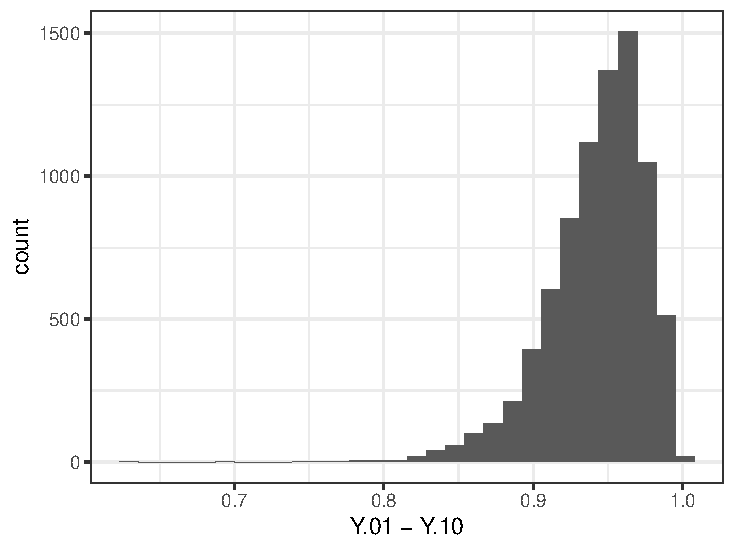
\includegraphics[width=0.6\textwidth,height=\textheight]{paper_files/figure-pdf/fig-posterior-dist-1.pdf}

}

\caption{\label{fig-posterior-dist}Posterior on ``Probability \(Y\) is
increasing in \(X\)''.}

\end{figure}%

\FloatBarrier

\subsubsection{Query distribution}\label{query-distribution}

It is generally helpful to use causal syntax to define the query and
calculate the query with respect to the prior or posterior probability
distributions. This can be done for a list of queries using
\texttt{query\_distribution()} function as follows:

\begin{verbatim}
R> queries <- 
+  make_model("X -> Y") |> 
+  query_distribution(
+    query = list(increasing = "(Y[X=1] > Y[X=0])",
+                 ATE = "(Y[X=1] - Y[X=0])"), 
+    using = "priors")
\end{verbatim}

The command \texttt{query\_distribution()} can also be used when one is
interested in assessing the value of a query for a \emph{particular
case}. In a sense, this is equivalent to posing a conditional query,
querying conditional on values in a case. For instance, we might consult
our posterior for the Lipids model and ask about the effect of \(X\) on
\(Y\) for a case in which \(Z=1\), \(X=1\) and \(Y=1\).

\begin{verbatim}
R> lipids_model |>
+  query_model(query = "Y[X=1] - Y[X=0]",
+              given = "X==1 & Y==1 & Z==1",
+              using = "posteriors")  |> 
+  subset(select = c("query", "mean", "sd"))
\end{verbatim}

\begin{verbatim}
#> 
#> Causal queries generated by query_model
#> 
#> |query           |  mean|   sd|
#> |:---------------|-----:|----:|
#> |Y[X=1] - Y[X=0] | 0.496| 0.24|
\end{verbatim}

The result is what we should now believe for all cases in which \(Z=1\),
\(X=1\), and \(Y=1\). It is the expected average effect among cases with
this data type, so this expectation has an uncertainty attached
reflecting our uncertainty about the expectation.

This is, in principle, different from what we would infer if we were
presented with a new case. When inquiring about a new case, we need to
\emph{update} on the given information observed in the new case. This
\emph{new} case-level inference is calculated if the
\texttt{case\_level\ =\ TRUE} argument is specified. For a query \(Q\)
and given \(D\) this returns the value
\(\frac{\int\pi(Q \& D | \lambda_i)p(\lambda_i)d\lambda_i}{\int\pi(D | \lambda_i)p(\lambda_i)d\lambda_i}\)
which may differ from the mean of the distribution
\(\frac{\pi(Q \& D | \lambda)}{\pi(D | \lambda)}\),
\(\int \frac{\pi(Q \& D | \lambda_i)}{\pi(D | \lambda_i)} p(\lambda_i)d\lambda_i\).

To illustrate the difference, consider an
\(X \rightarrow M \rightarrow Y\) model where we are quite certain that
\(X\) causes \(Y\), but unsure whether this effect works through two
positive or two negative effects. If asked what we would think about
effects in cases \(M=0\) (or with \(M=1\)), we have little basis to know
whether these are cases in which effects are more or less likely.
However, if we randomly find a case and we observe that \(M=0\), our
understanding of the causal model evolves, leading us to believe there
is (or is not) an effect in this specific case. The case-level query
gives a single value without posterior standard deviation, representing
the belief about this new case.

\begin{verbatim}
R> make_model("X -> M -> Y") |>
+  update_model(data.frame(X = rep(0:1, 8), Y = rep(0:1, 8)), iter = 4000) |>
+  query_model("Y[X=1] > Y[X=0]", 
+            given = "X==1 & Y==1 & M==1", 
+            using = "posteriors",
+            case_level = c(TRUE, FALSE))  |> 
+  subset(select = c("query", "case_level", "mean", "sd"))
\end{verbatim}

\begin{verbatim}
#> 
#> Causal queries generated by query_model
#> 
#> |query           |case_level |  mean|    sd|
#> |:---------------|:----------|-----:|-----:|
#> |Y[X=1] > Y[X=0] |TRUE       | 0.673|    NA|
#> |Y[X=1] > Y[X=0] |FALSE      | 0.424| 0.327|
\end{verbatim}

\subsubsection{Batch queries}\label{batch-queries}

The function \texttt{query\_model()} can also be used to query multiple
models. The function takes a list of models, causal queries, and
conditions as inputs. It then calculates population or case level
estimands given prior or posterior distributions and reports summaries
of these distributions. The result is a data frame that can be displayed
as a table or used for graphing.

Table~\ref{tbl-batch-query} returns to the Lipids data and shows the
output from a single call to \texttt{query\_model()} with the
\texttt{expand\_grid} argument set to \texttt{TRUE} to generate all
combinations of list elements.

\begin{verbatim}
R> models <- list(
+  A = lipids_model |> 
+    update_model(data = lipids_data, refresh = 0),
+  B = lipids_model |> set_restrictions("X[Z=1] < X[Z=0]") |>
+    update_model(data = lipids_data, refresh = 0))
R> 
R> queries <- 
+  query_model(
+    models,  
+    query = list(ATE = "Y[X=1] - Y[X=0]", 
+                 POS = "Y[X=1] > Y[X=0]"),
+    given = c(TRUE,  "Y==1 & X==1"),
+    case_level = c(FALSE, TRUE),
+    using = c("priors", "posteriors"),
+    expand_grid = TRUE)
\end{verbatim}

\begin{longtable}[t]{ccccccc}

\caption{\label{tbl-batch-query}Results for two queries on two models.}

\tabularnewline

\toprule
model & query & given & using & case\_level & mean & sd\\
\midrule
A & ATE & - & priors & FALSE & 0.00 & 0.20\\
B & ATE & - & priors & FALSE & 0.00 & 0.23\\
A & ATE & - & posteriors & FALSE & 0.55 & 0.10\\
B & ATE & - & posteriors & FALSE & 0.56 & 0.10\\
A & ATE & Y==1 \& X==1 & priors & FALSE & 0.50 & 0.22\\
\addlinespace
B & ATE & Y==1 \& X==1 & priors & FALSE & 0.49 & 0.24\\
A & ATE & Y==1 \& X==1 & posteriors & FALSE & 0.95 & 0.04\\
B & ATE & Y==1 \& X==1 & posteriors & FALSE & 0.95 & 0.04\\
A & POS & - & priors & FALSE & 0.25 & 0.12\\
B & POS & - & priors & FALSE & 0.25 & 0.14\\
\addlinespace
A & POS & - & posteriors & FALSE & 0.61 & 0.10\\
B & POS & - & posteriors & FALSE & 0.61 & 0.10\\
A & POS & Y==1 \& X==1 & priors & FALSE & 0.50 & 0.22\\
B & POS & Y==1 \& X==1 & priors & FALSE & 0.49 & 0.24\\
A & POS & Y==1 \& X==1 & posteriors & FALSE & 0.95 & 0.04\\
\addlinespace
B & POS & Y==1 \& X==1 & posteriors & FALSE & 0.95 & 0.04\\
A & ATE & - & priors & TRUE & 0.00 & NA\\
B & ATE & - & priors & TRUE & 0.00 & NA\\
A & ATE & - & posteriors & TRUE & 0.55 & NA\\
B & ATE & - & posteriors & TRUE & 0.56 & NA\\
\addlinespace
A & ATE & Y==1 \& X==1 & priors & TRUE & 0.50 & NA\\
B & ATE & Y==1 \& X==1 & priors & TRUE & 0.49 & NA\\
A & ATE & Y==1 \& X==1 & posteriors & TRUE & 0.95 & NA\\
B & ATE & Y==1 \& X==1 & posteriors & TRUE & 0.95 & NA\\
A & POS & - & priors & TRUE & 0.25 & NA\\
\addlinespace
B & POS & - & priors & TRUE & 0.25 & NA\\
A & POS & - & posteriors & TRUE & 0.61 & NA\\
B & POS & - & posteriors & TRUE & 0.61 & NA\\
A & POS & Y==1 \& X==1 & priors & TRUE & 0.50 & NA\\
B & POS & Y==1 \& X==1 & priors & TRUE & 0.49 & NA\\
\addlinespace
A & POS & Y==1 \& X==1 & posteriors & TRUE & 0.95 & NA\\
B & POS & Y==1 \& X==1 & posteriors & TRUE & 0.95 & NA\\
\bottomrule

\end{longtable}

\section{Conclusion}\label{conclusion}

M TO ADD TEXT HERE

\FloatBarrier

\newpage{}

\section*{Computational details and software
requirements}\label{computational-details-and-software-requirements}
\addcontentsline{toc}{section}{Computational details and software
requirements}

\begin{longtable}[]{@{}
  >{\raggedleft\arraybackslash}p{(\columnwidth - 2\tabcolsep) * \real{0.3000}}
  >{\raggedright\arraybackslash}p{(\columnwidth - 2\tabcolsep) * \real{0.7000}}@{}}
\toprule\noalign{}
\endhead
\bottomrule\noalign{}
\endlastfoot
Version & \begin{minipage}[t]{\linewidth}\raggedright
\begin{itemize}
\tightlist
\item
  1.1.1
\end{itemize}
\end{minipage} \\
Availability & \begin{minipage}[t]{\linewidth}\raggedright
\begin{itemize}
\tightlist
\item
  Stable Release:
  \url{https://cran.rstudio.com/web/packages/CausalQueries/index.html}
\item
  Development:
  \url{https://github.com/integrated-inferences/CausalQueries}
\end{itemize}
\end{minipage} \\
Issues & \begin{minipage}[t]{\linewidth}\raggedright
\begin{itemize}
\tightlist
\item
  \url{https://github.com/integrated-inferences/CausalQueries/issues}
\end{itemize}
\end{minipage} \\
Operating Systems & \begin{minipage}[t]{\linewidth}\raggedright
\begin{itemize}
\tightlist
\item
  Linux
\item
  MacOS
\item
  Windows
\end{itemize}
\end{minipage} \\
Testing Environments OS & \begin{minipage}[t]{\linewidth}\raggedright
\begin{itemize}
\tightlist
\item
  Ubuntu 22.04.2
\item
  Debian 12.2
\item
  MacOS
\item
  Windows
\end{itemize}
\end{minipage} \\
Testing Environments R & \begin{minipage}[t]{\linewidth}\raggedright
\begin{itemize}
\tightlist
\item
  R 4.3.1
\item
  R 4.3.0
\item
  R 4.2.3
\item
  r-devel
\end{itemize}
\end{minipage} \\
R Version & \begin{minipage}[t]{\linewidth}\raggedright
\begin{itemize}
\tightlist
\item
  R(\textgreater= 3.4.0)
\end{itemize}
\end{minipage} \\
Compiler & \begin{minipage}[t]{\linewidth}\raggedright
\begin{itemize}
\tightlist
\item
  either of the below or similar:
\item
  g++
\item
  clang++
\end{itemize}
\end{minipage} \\
Stan requirements & \begin{minipage}[t]{\linewidth}\raggedright
\begin{itemize}
\tightlist
\item
  inline
\item
  Rcpp (\textgreater= 0.12.0)
\item
  RcppEigen (\textgreater= 0.3.3.3.0)
\item
  RcppArmadillo (\textgreater= 0.12.6.4.0)
\item
  RcppParallel (\textgreater= 5.1.4)
\item
  BH (\textgreater= 1.66.0)
\item
  StanHeaders (\textgreater= 2.26.0)
\item
  rstan (\textgreater= 2.26.0)
\end{itemize}
\end{minipage} \\
R-Packages Depends & \begin{minipage}[t]{\linewidth}\raggedright
\begin{itemize}
\tightlist
\item
  dplyr
\item
  methods
\end{itemize}
\end{minipage} \\
R-Packages Imports & \begin{minipage}[t]{\linewidth}\raggedright
\begin{itemize}
\tightlist
\item
  dagitty (\textgreater= 0.3-1)
\item
  dirmult (\textgreater= 0.1.3-4)
\item
  stats (\textgreater= 4.1.1)
\item
  rlang (\textgreater= 0.2.0)
\item
  rstan (\textgreater= 2.26.0)
\item
  rstantools (\textgreater= 2.0.0)
\item
  stringr (\textgreater= 1.4.0)
\item
  ggdag (\textgreater= 0.2.4)
\item
  latex2exp (\textgreater= 0.9.4)
\item
  ggplot2 (\textgreater= 3.3.5)
\item
  lifecycle (\textgreater= 1.0.1)
\end{itemize}
\end{minipage} \\
\end{longtable}

The results in this paper were obtained using
\proglang{R}\textasciitilde3.4.1 with the
\pkg{MASS}\textasciitilde7.3.47 package. \proglang{R} itself and all
packages used are available from the Comprehensive \proglang{R} Archive
Network (CRAN) at \url{https://CRAN.R-project.org/}.

\section*{Acknowledgments}\label{acknowledgments}
\addcontentsline{toc}{section}{Acknowledgments}

\begin{tcolorbox}[enhanced jigsaw, bottomrule=.15mm, leftrule=.75mm, opacityback=0, breakable, arc=.35mm, colframe=quarto-callout-color-frame, rightrule=.15mm, colback=white, left=2mm, toprule=.15mm]

We thank Ben Goodrich, who provided generous insights on using
\texttt{stan} for this project. We thank Alan M Jacobs for key work in
developing the framework underlying the package. Our thanks to
Cristian-Liviu Nicolescu, who provided wonderful feedback on the use of
the package and a draft of this paper. Our thanks to Jasper Cooper for
contributions to the generic function to create Stan code, to
\href{https://clarabicalho.github.io/}{Clara Bicalho}, who helped figure
out the syntax for causal statements, to
\href{https://www.gov.harvard.edu/directory/julio-s-solis-arce/}{Julio
S. Solís Arce} who made many vital contributions figuring out how to
simplify the specification of priors, and to
\href{https://merlinheidemanns.github.io/website/}{Merlin Heidemanns}
who figured out the \texttt{rstantools} integration and made myriad code
improvements.

\end{tcolorbox}

\section*{References}\label{references}
\addcontentsline{toc}{section}{References}

\renewcommand{\bibsection}{}
\bibliography{supp/cq_jss.bib}

\newpage{}

\section*{Appendix A: Parallelization}\label{sec-parallel}
\addcontentsline{toc}{section}{Appendix A: Parallelization}

If users have access to multiple cores, parallel processing can be
implemented by including this line before running
\texttt{CausalQueries}:

\begin{verbatim}
R> library(parallel)
R> 
R> options(mc.cores = parallel::detectCores())
\end{verbatim}

Additionally, parallelizing across models or data while running MCMC
chains in parallel can be achieved by setting up a nested parallel
process. With 8 cores one can run two updating processes with three
parallel chains each simultaneously. More generally the number of
parallel processes at the upper level of the nested parallel structure
are given by \(\left \lfloor \frac{cores}{chains + 1} \right \rfloor\).

\begin{verbatim}
R> library(future)
R> library(future.apply)
R> 
R> chains <- 3
R> cores <- 8
R> 
R> future::plan(list(
+      future::tweak(future::multisession, 
+                    workers = floor(cores/(chains + 1))),
+      future::tweak(future::multisession, 
+                    workers = chains)
+    ))
R> 
R> model <- make_model("X -> Y")
R> data <- list(data_1 = data.frame(X=0:1, Y=0:1), 
+             data_2 = data.frame(X=0:1, Y=1:0))
R> 
R> results <-
+future.apply::future_lapply(
+  data,
+  function(d) {
+    update_model(
+      model = model,
+      data = d,
+      chains = chains,
+      refresh = 0
+    )},
+ future.seed = TRUE)
\end{verbatim}

\newpage

\section*{Appendix B: Stan code}\label{sec-stancode}
\addcontentsline{toc}{section}{Appendix B: Stan code}

Updating is performed using a generic Stan model. The data provided to
Stan is generated by the internal function \texttt{prep\_stan\_data()},
which returns a list of objects that Stan expects to receive. The code
for the Stan model is shown below. After defining a helper function, the
code starts with a block declaring what input data is to be expected.
Then, the parameters and the transformed parameters are characterized.
Then, the likelihoods and priors are provided. At the end, a block for
generated quantities is used to append a posterior distribution of
causal types to the model.

\begin{verbatim}
S4 class stanmodel 'simplexes' coded as follows:
functions{
  row_vector col_sums(matrix X) {
    row_vector[cols(X)] s ;
    s = rep_row_vector(1, rows(X)) * X ;
    return s ;
  }
}
data {
int<lower=1> n_params;
int<lower=1> n_paths;
int<lower=1> n_types;
int<lower=1> n_param_sets;
int<lower=1> n_nodes;
array[n_param_sets] int<lower=1> n_param_each;
int<lower=1> n_data;
int<lower=1> n_events;
int<lower=1> n_strategies;
int<lower=0, upper=1> keep_type_distribution;
vector<lower=0>[n_params] lambdas_prior;
array[n_param_sets] int<lower=1> l_starts;
array[n_param_sets] int<lower=1> l_ends;
array[n_nodes] int<lower=1> node_starts;
array[n_nodes] int<lower=1> node_ends;
array[n_strategies] int<lower=1> strategy_starts;
array[n_strategies] int<lower=1> strategy_ends;
matrix[n_params, n_types] P;
matrix[n_params, n_paths] parmap;
matrix[n_paths, n_data] map;
matrix<lower=0,upper=1>[n_events,n_data] E;
array[n_events] int<lower=0> Y;
}
parameters {
vector<lower=0>[n_params - n_param_sets] gamma;
}
transformed parameters {
vector<lower=0, upper=1>[n_params] lambdas;
vector<lower=1>[n_param_sets] sum_gammas;
matrix[n_params, n_paths] parlam;
matrix[n_nodes, n_paths] parlam2;
vector<lower=0, upper=1>[n_paths] w_0;
vector<lower=0, upper=1>[n_data] w;
vector<lower=0, upper=1>[n_events] w_full;
// Cases in which a parameter set has only one value need special handling
// they have no gamma components and sum_gamma needs to be made manually
for (i in 1:n_param_sets) {
  if (l_starts[i] >= l_ends[i]) {
    sum_gammas[i] = 1;
    lambdas[l_starts[i]] = 1;
    }
  else if (l_starts[i] < l_ends[i]) {
    sum_gammas[i] =
    1 + sum(gamma[(l_starts[i] - (i-1)):(l_ends[i] - i)]);
    lambdas[l_starts[i]:l_ends[i]] =
    append_row(1, gamma[(l_starts[i] - (i-1)):(l_ends[i] - i)]) /
      sum_gammas[i];
    }
  }
// Mapping from parameters to data types
// (usual case): [n_par * n_data] * [n_par * n_data]
parlam  = rep_matrix(lambdas, n_paths) .* parmap;
// Sum probability over nodes on each path
for (i in 1:n_nodes) {
 parlam2[i,] = col_sums(parlam[(node_starts[i]):(node_ends[i]),]);
 }
// then take product  to get probability of data type on path
for (i in 1:n_paths) {
  w_0[i] = prod(parlam2[,i]);
 }
 // last (if confounding): map to n_data columns instead of n_paths
 w = map'*w_0;
  // Extend/reduce to cover all observed data types
 w_full = E * w;
}
model {
// Dirichlet distributions
for (i in 1:n_param_sets) {
  target += dirichlet_lpdf(lambdas[l_starts[i]:l_ends[i]]  |
    lambdas_prior[l_starts[i] :l_ends[i]]);
  target += -n_param_each[i] * log(sum_gammas[i]);
 }
// Multinomials
// Note with censoring event_probabilities might not sum to 1
for (i in 1:n_strategies) {
  target += multinomial_lpmf(
  Y[strategy_starts[i]:strategy_ends[i]] |
    w_full[strategy_starts[i]:strategy_ends[i]]/
     sum(w_full[strategy_starts[i]:strategy_ends[i]]));
 }
}
// Option to export distribution of causal types
generated quantities{
vector[n_types] types;
if (keep_type_distribution == 1){
for (i in 1:n_types) {
   types[i] = prod(P[, i].*lambdas + 1 - P[,i]);
}}
 if (keep_type_distribution == 0){
    types = rep_vector(1, n_types);
 }
} 
\end{verbatim}

\newpage

\section*{Appendix C: Benchmarks}\label{sec-benchmark}
\addcontentsline{toc}{section}{Appendix C: Benchmarks}

We present a brief summary of model updating benchmarks. Note that these
benchmarks are not generally reproducible and depend on the
specifications of the hardware system used to produce them. The first
benchmark considers the effect of model complexity on updating time. The
second benchmark considers the effect of data size on updating time. We
run four parallel chains for each model. The results of the benchmarks
are presented in Table~\ref{tbl-bench1} and Table~\ref{tbl-bench2}.

\begin{longtable}[]{@{}
  >{\centering\arraybackslash}p{(\columnwidth - 4\tabcolsep) * \real{0.4000}}
  >{\centering\arraybackslash}p{(\columnwidth - 4\tabcolsep) * \real{0.3000}}
  >{\centering\arraybackslash}p{(\columnwidth - 4\tabcolsep) * \real{0.3000}}@{}}
\caption{Benchmark 1.}\label{tbl-bench1}\tabularnewline
\toprule\noalign{}
\begin{minipage}[b]{\linewidth}\centering
Model
\end{minipage} & \begin{minipage}[b]{\linewidth}\centering
Number of Model Parameters
\end{minipage} & \begin{minipage}[b]{\linewidth}\centering
\texttt{update\_model()} Run-Time (seconds)
\end{minipage} \\
\midrule\noalign{}
\endfirsthead
\toprule\noalign{}
\begin{minipage}[b]{\linewidth}\centering
Model
\end{minipage} & \begin{minipage}[b]{\linewidth}\centering
Number of Model Parameters
\end{minipage} & \begin{minipage}[b]{\linewidth}\centering
\texttt{update\_model()} Run-Time (seconds)
\end{minipage} \\
\midrule\noalign{}
\endhead
\bottomrule\noalign{}
\endlastfoot
\(X1 \rightarrow Y\) & 6 & 7.0 \\
\(X1 \rightarrow Y; X2 \rightarrow Y\) & 20 & 8.4 \\
\(X1\rightarrow Y;X2\rightarrow Y;X3\rightarrow Y\) & 262 & 22.9 \\
\end{longtable}

\begin{longtable}[]{@{}
  >{\centering\arraybackslash}p{(\columnwidth - 4\tabcolsep) * \real{0.4000}}
  >{\centering\arraybackslash}p{(\columnwidth - 4\tabcolsep) * \real{0.3000}}
  >{\centering\arraybackslash}p{(\columnwidth - 4\tabcolsep) * \real{0.3000}}@{}}
\caption{Benchmark 2.}\label{tbl-bench2}\tabularnewline
\toprule\noalign{}
\begin{minipage}[b]{\linewidth}\centering
Model
\end{minipage} & \begin{minipage}[b]{\linewidth}\centering
Number of Observations
\end{minipage} & \begin{minipage}[b]{\linewidth}\centering
\texttt{update\_model()} Run-Time (seconds) \textbar{}
\end{minipage} \\
\midrule\noalign{}
\endfirsthead
\toprule\noalign{}
\begin{minipage}[b]{\linewidth}\centering
Model
\end{minipage} & \begin{minipage}[b]{\linewidth}\centering
Number of Observations
\end{minipage} & \begin{minipage}[b]{\linewidth}\centering
\texttt{update\_model()} Run-Time (seconds) \textbar{}
\end{minipage} \\
\midrule\noalign{}
\endhead
\bottomrule\noalign{}
\endlastfoot
\(X1 \rightarrow Y\) & 10 & 5.8 \\
\(X1 \rightarrow Y\) & 100 & 6.5 \\
\(X1 \rightarrow Y\) & 1000 & 7.0 \\
\(X1 \rightarrow Y\) & 10000 & 10.6 \\
\(X1 \rightarrow Y\) & 100000 & 22.9 \\
\end{longtable}

Increasing the number of parents in a model greatly increases the number
of parameters and computational time. The results suggests the
computational time is convex in the number of parents and approximately
linear in the number of parameters. Unless model restrictions are
imposed four parents would yield 65,536 parameters. The rapid growth of
the parameter space with increasing model complexity places limits on
feasible computability without further recourse to specialized methods
for handling large causal models. In contrast, the results suggest that
computational time is concave in the size of the data.




\end{document}
